\chapter{Beyond the Standard Model}
\label{chapter:BSM}

This chapter describes several extensions of the Standard Model.
These extensions aim to solve some of the many aspects of Nature that the SM cannot explain.
In particular, supersymmetry, the Arkani-Hamed Dvali Dimopoulos model of Large Extra Dimensions, and some models involving the production of Dark Matter will be covered in the following.


\section{Motivation to go beyond the Standard Model}
\label{sec:MotivationBSM}

The Standard Model provides the most successful description of the leptons, quarks and the interactions between them through the different bosons, as it was discussed throughout Chapter \ref{chapter:StandardModel}.
For the moment, no experiment besides the neutrino oscillations, that reveal the massive character of the neutrinos, has been able to find any clear deviation of the data with respect to the SM predictions.
However, there are a number of physical arguments that point to the existence of a theory that extends the SM in order to describe the physics at higher energies.

The first argument comes from the fact that gravity is not accommodated in the theory, thus preventing the Standard Model to be the Theory Of Everything (TOE), in which Nature could be described in a single framework.
For this reason, a new model is required at the reduced Planck scale $M_P = \left(8\pi G_\text{Newton}\right)^{-1/2} = \unit[2.4\times 10^{18}]{GeV}$, where the quantum gravitational effects are not negligible.

A further argument pointing to the need for new theories beyond the SM is the ``hierarchy problem'', regarded as a consequence of the fact that the ratio $M_P/M_W$ is so huge.
This is not a difficulty with the Standard Model itself, but rather a disturbing sensitivity of the Higgs potential to new physics in almost any imaginable extension of the SM.
Unlike the fermions and gauge bosons, spin-0 fields are not protected by any chiral or gauge symmetries against large radiative corrections to their masses.
In particular, in the SM there is no mechanism to prevent scalar particles from acquiring large masses through radiative corrections.
For this reason, the Higgs field receives enormous corrections from the virtual effects of any SM particle it couples to (see fermion loop diagram from Figure \ref{fig:HiggsLoop}).

\begin{figure}[!t]
\begin{center}
\mbox{
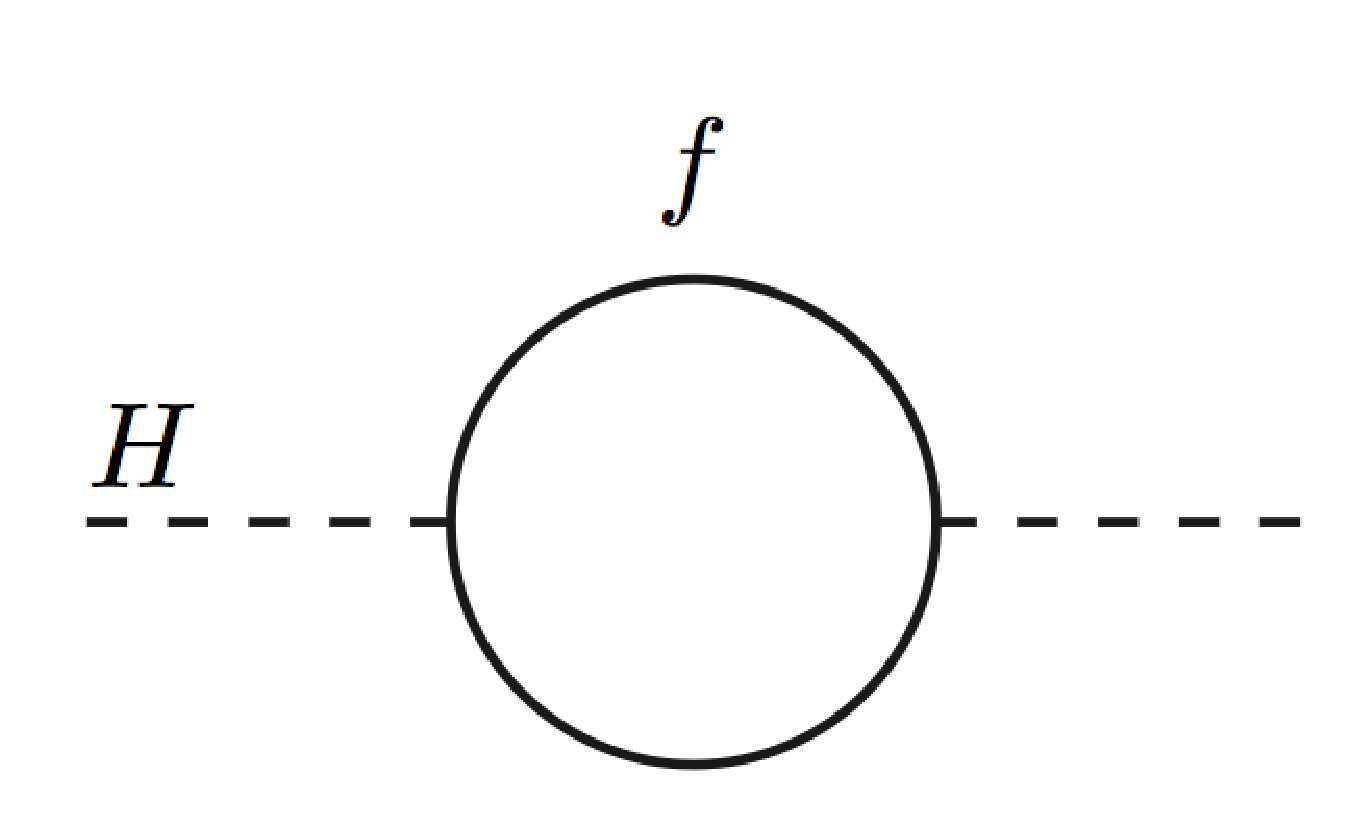
\includegraphics[width=0.495\textwidth]{BeyondSM/Figures/HiggsLoopFermion.eps}
%        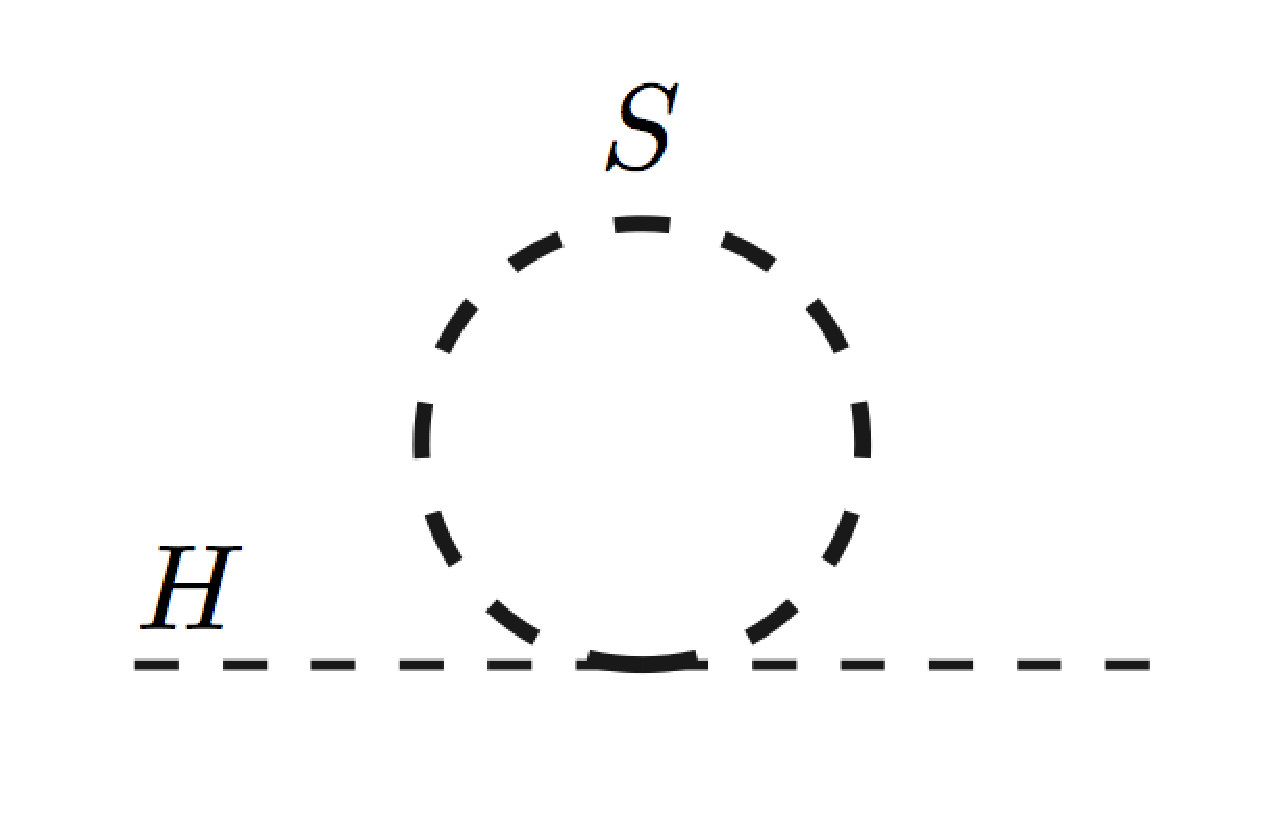
\includegraphics[width=0.495\textwidth]{BeyondSM/Figures/HiggsLoopScalar.eps}
}
\end{center}
\caption{One-loop quantum corrections to the Higgs mass due to fermions.}
\label{fig:HiggsLoop}
\end{figure}

Due to these corrections, the Higgs mass is:

\begin{equation}
m_{H_{\text{SM}}}^2 = (m_H)_{0}^{2} + \Delta m_H^2,
\label{eq:HiggsMassTotal}
\end{equation}

\noindent where $(m_H)_0$ is the bare Higgs mass and $\Delta m_H^2$ is the Higgs mass correction which, for the case of a fermion loop, is given by:

\begin{equation}
\Delta m_H^2 = -\frac{|\lambda_f|^2}{16\pi^2}\left[2\Lambda^2 + \mathcal{O}\left(m_f^2\ln{\left(\frac{\Lambda}{m_f}\right)}\right)\right],
\label{eq:HiggsMassCorrectionFermion}
\end{equation}

\noindent being $\lambda_f$ the Yukawa coupling of the fermion $f$ and being $\Lambda$ a cutoff.
The latter is interpreted as the energy scale at which new physics enters and the SM ceases to be valid.
If the SM needs to describe Nature up to $M_P$, then the quantum corrections to the Higgs mass can be as big as 30 orders of magnitude larger than the Higgs mass squared.
The cancellation of these corrections at all orders would imply an enormous \emph{fine tuning} in order to recover the measured mass of the Higgs boson.
In a model with spontaneous electroweak symmetry breaking, this problem also affects other particles that get their masses through this mechanism, such as the $W$, the $Z$, the quarks and the charged leptons.
It is therefore unnatural to have all the SM particle masses at the electroweak scale unless they are ``forced'' to be in this range due to a cutoff of the Standard Model in much lower energies than the Planck scale.

Even accepting the fine tuning required in order to keep the SM particle masses at the order of the electroweak scale, the SM contains 19 free parameters, such as couplings, masses and mixings, which cannot be predicted theoretically but must be measured by the experiment.
In addition to it, more parameters would be needed in order to accommodate non-accelerator observations, such as neutrino masses and mixings.
Another reason to look for physics beyond the Standard Model is related to the nature of the \emph{Dark Matter}, whose existence is inferred from cosmological observations such as studies on the Cosmic Microwave Background or the rotation pattern of the galaxies, for which there are no candidates among the SM particles.

The Standard Model also leaves other questions unanswered, such as why there are three generations of quarks and leptons or three colors; why proton and electron electric charges are exactly opposite; which is the origin of the matter-antimatter asymmetry observed in the Universe; the relation between strong and electroweak forces, or the origin of the neutrino masses.

Along the years, many theories have been developed in order to give an explanation to the items mentioned above.
In the following sections, three scenarios for physics beyond the SM will be reviewed.
They are of particular interest for this Thesis, because they predict new phenomena that leads to monojet final state signatures and could be observable in the energy reach of the LHC.


\section{Supersymmetry}
\label{sec:SUSY}

The hierarchy problem introduced in the previous section can be elegantly solved if for each SM fermion, a new boson $S$ is introduced in a way that it also couples to the Higgs.
This new scalar would translate into a mass correction term of the form:

\begin{equation}
\Delta m_H^2 = \frac{\lambda_f^2}{16\pi^2}\left[2\Lambda^2 + \mathcal{O}\left(m_S^2\ln{\left(\frac{\Lambda}{m_S}\right)}\right)\right].
\label{eq:HiggsMassCorrectionScalar}
\end{equation}

Fermi statistics implies an opposite sign with respect to the fermion mass correction shown in Equation \ref{eq:HiggsMassCorrectionFermion}.
Therefore, if $\lambda_S = |\lambda_f|$, all the fermion terms have a counter term that naturally cancels the quadratic divergence introduced.
Therefore, assuming the existence of this scalar partner, the remaining terms in the Higgs mass correction are:

\begin{equation}
\Delta m_H^2 = \frac{\lambda_f^2}{16\pi^2} |m_S^2 - m_f^2|,
\label{eq:HiggsMassCorrectionNoQuadratic}
\end{equation}

\noindent where the smaller logarithmic contributions have been omitted.
According to the the ``Naturalness'' argument \cite{Witten:1981nf}, these corrections must not be much greater than $m_{H_{\text{SM}}}$ in order to avoid too much fine tuning.
If so,

\begin{equation}
|m_S^2 - m_f^2| \lesssim \unit[1]{TeV}^2,
\label{eq:HiggsNaturalnessCondition}
\end{equation}

\noindent which sets the scale of validity of the SM to be of the order of the TeV.
At higher scales, new particles would be produced and thus the SM should be substituted by its supersymmetric extension, which would be valid up to the Planck scale.

The following subsections introduce the foundations of supersymmetric lagrangians, in order to obtain a recipe to write down the allowed interactions and mass terms of a general supersymmetric theory.
This recipe will be then applied to the special case of the Minimal Supersymmetric Standard Model.
Finally, the gauge mediated supersymmetry breaking framework will be discussed.


\subsection{Building a general supersymmetric lagrangian}

A supersymmetry (SUSY) transformation turns a bosonic state into a fermionic state and vice versa~\cite{Drees:1996ca}:

\begin{equation}
\hat{Q} |\text{Boson}\rangle = |\text{Fermion}\rangle \;\;\;\text{and}\;\;\; \hat{Q} |\text{Fermion}\rangle = |\text{Boson}\rangle
\label{eq:SUSYGeneralTransformation}
\end{equation}

\noindent where the operator $\hat{Q}$ is the generator of the SUSY transformation.
It must be an anticommuting spinor and since spinors are intrinsically complex objects, $Q^\dagger$ is also a symmetry generator, which satisfies a Lie algebra~\cite{Haag}.
Since $Q$ and $Q^\dagger$ are fermionic operators, they carry spin $1/2$, thus making clear that SUSY is a spacetime symmetry.
In fact, SUSY seems to be the last possible extension of the Lorentz group \cite{Haag2}.
In the notation used in the following, SM particles are combined to supersymmetric particles into superfields.


\subsubsection{Chiral supermultiplets}

In a realistic theory, there are many chiral supermultiplets, with both gauge and non-gauge interactions.
The lagrangian density for a collection of free chiral supermultiplets labeled by the index $i$ is shown in Equation \ref{eq:SUSYIntroGeneralAction},

\begin{equation}
\begin{split}
&\lagrangian_{\text{chiral}} = \lagrangian_{\text{chiral, scalar}} + \lagrangian_{\text{chiral, fermion}}, \text{     being  } \\
&\lagrangian_{\text{chiral, scalar}} = - \partial^{\mu} \phi^{\ast i} \partial_{\mu} \phi_i \text{      and  } \\
&\lagrangian_{\text{chiral, fermion}} = i\psi^{\dagger i} \bar{\sigma}^\mu \partial_{\mu} \psi_i ,
\end{split}
\label{eq:SUSYIntroGeneralAction}
\end{equation}

\noindent where $\sigma^\mu$ are the Pauli matrices.
If the lagrangian in Equation \ref{eq:SUSYIntroGeneralAction} is invariant under supersymmetry transformations, it must be satisfied that $\delta S = 0$, thus requiring the fields of the theory to transform as:

%\begin{equation}
\begin{align}
\delta \phi_i &= \epsilon \psi_i  &  \delta \phi^{\ast i} &= \epsilon^\dagger \psi^{\dagger i} \\
\delta (\psi_i)_\alpha &= -i(\sigma^\mu \epsilon^{\dagger})_\alpha \partial_\mu \phi_i + \epsilon_\alpha F_i, & \delta (\psi^{\dagger i})_\alpha &= i(\epsilon \sigma^\mu)_\alpha \partial_\mu \phi^{\ast i} + \epsilon^{\dagger}_\alpha F^{\ast i} \\
\delta F_i &= -i\epsilon^\dagger \bar{\sigma}^\mu \partial_\mu \psi_i, & \delta F^{\ast i} &= i\partial_\mu \psi^{\dagger i} \bar{\sigma}^\mu \epsilon.
\label{eq:SUSYFieldsTransformation}
\end{align}
%\end{equation}

The auxiliary fields $F_i$ need to be introduced to make supersymmetry exact off-shell.
Each auxiliary field satisfies the following lagrangian, to be added to Equation \ref{eq:SUSYIntroGeneralAction}:

\begin{equation}
\lagrangian_\text{chiral, auxiliary} = F^{\ast i} F_i,
\label{eq:SUSYChiralAuxiliaryLagrangian}
\end{equation}

\noindent which implies the equations of motion $F_i=0$ and $F^{\ast i}=0$, thus vanishing on-shell.
In fact, each complex scalar field $\phi_i$ has two real propagating degrees of freedom, matching the two spin polarizations of its corresponding fermionic field $\psi_i$, on-shell.
Off-shell, however, the fermionic field is a complex two-component object, so it has four degrees of freedom.
To make the degrees of freedom for the fermionic and bosonic fields match, the auxiliary field $F_i$ needs to be introduced.
The counting of real degrees of freedom in this simplified model is shown in Table \ref{tab:SUSYChiralCountingDOF}.

\begin{table}[!ht]
\begin{center}
\begin{small}
\begin{tabular}{cccc}
\hline
\hline
& $\phi_i$ & $\psi_i$ & $F_i$ \\
\hline
on-shell ($n_B = n_F = 2$)  & 2      & 2      & 0 \\
off-shell ($n_B = n_F = 4$) & 2      & 4      & 2 \\
\hline
\hline
\end{tabular}
\end{small}
\end{center}
\caption{Counting of real degrees of freedom in supersymmetric theories.}
\label{tab:SUSYChiralCountingDOF}
\end{table}

On the other hand, the most general set of renormalizable interactions for these fields that is consistent with supersymmetry is found to be \cite{Martin:1997ns}:

\begin{equation}
\lagrangian_{\text{chiral, int}} = \left( -\frac{1}{2} W^{ij}\psi_i \psi_j + W^i F_i\right) + c.c.
\label{eq:SUSYChiralInteractionLagrangian}
\end{equation}

\noindent where $W^{ij}$ and $W^i$ can be derived from the following superpotential:

\begin{equation}
W = \frac{1}{2} M^{ij} \phi_i \phi_j + \frac{1}{6} y^{ijk} \phi_i \phi_j \phi_k ,
\label{eq:SUSYChiralSuperpotential}
\end{equation}

\noindent with

\begin{equation}
\begin{split}
& W^{ij} = \frac{\delta^2}{\delta\phi_i \, \delta\phi_j} W \\
& W^{i} = \frac{\delta}{\delta\phi_i} W. \\
\end{split}
\label{eq:SUSYChiralSuperpotentialDerivations}
\end{equation}

If the interaction lagrangian from Equation \ref{eq:SUSYChiralInteractionLagrangian} is added to the chiral lagrangian from equation \ref{eq:SUSYIntroGeneralAction}, the part that contains the auxiliary fields leads to the equations of motion $F_i = - W^{\ast}_i$ and $F^{\ast i} = - W^i$ and the auxiliary fields can be expressed algebraically in terms of the scalar fields.
Therefore, after the non-propagating fields $F_i$ and $F^{\ast i}$ have been eliminated, the full lagrangian density for the chiral fields is found to be:

\begin{equation}
\begin{split}
\lagrangian_{\text{chiral}} = & -\partial^\mu \phi^{\ast i} \partial_\mu \phi_i - V_\text{chiral}(\phi, \phi^{\ast}) + i\psi^{\dagger i}\bar{\sigma}^\mu \partial_\mu \psi_i \\
& - \frac{1}{2}M^{ij}\psi_i\psi_j - \frac{1}{2}M^{\ast}_{ij} \psi^i \psi^j \\
& - \frac{1}{2}y^{ijk}\psi_i \psi_j \psi_k - \frac{1}{2}y^{\ast}_{ijk}\psi^{\ast i} \psi^{\dagger j} \psi^{\dagger k},
\end{split}
\label{eq:SUSYChiralFinalLagrangian}
\end{equation}

\noindent with the chiral scalar potential $V_\text{chiral}(\phi, \phi^{\ast})$ defined as:

\begin{equation}
\begin{split}
V_\text{chiral}(\phi, \phi^{\ast}) = & W^k W^\ast_k = F^{\ast k} F_k = \\
& M^{\ast}_{ik} M^{kj} \phi^{\ast i} \phi_j + \frac{1}{2}M^{in} y^{\ast}_{jkn} \phi_i \phi^{\ast j} \phi^{\ast k} + \frac{1}{2}M^\ast_{in} y^{jkn} \phi^{\ast i} \phi_{j} \phi_{k} \\
& + \frac{1}{4} y^{ijk} y^{\ast}_{kln}\phi_i \phi_j \phi^{\ast k} \phi^{\ast l}.
\end{split}
\label{eq:SUSYChiralScalarPotential}
\end{equation}



\subsubsection{Gauge supermultiplets}

As it was already shown in Chapter \ref{chapter:StandardModel}, the global gauge symmetries can be promoted to local symmetries, which involves the presence of gauge fields.
The propagating degrees of freedom in a gauge supermultiplet are a massless gauge boson field $\vec{A}_\mu = A^\alpha_\mu$ and a two component Weyl Dirac gaugino $\vec{\lambda} = \lambda^\alpha$.
The gauge transformations of the vector supermultiplet fields are:

\begin{equation}
\begin{split}
&A^\alpha_\mu \rightarrow A'^\alpha_\mu = A^\alpha_\mu + \frac{1}{e}\partial_\mu \theta^\alpha + f^{\alpha \beta \gamma} A^\beta_\mu \theta_\gamma \\
&\lambda^\alpha \rightarrow \lambda'^\alpha = \lambda^\alpha + f^{\alpha \beta \gamma} \lambda^\beta \theta^\gamma,
\end{split}
\label{eq:SUSYGaugeTransformationFields}
\end{equation}

\noindent where $f^{\alpha \beta \gamma}$ are the totally antisymmetric structure constants that define the gauge group.
The special case of an Abelian group is obtained by just setting $f^{\alpha \beta \gamma} = 0$ (see Equation \ref{eq:QEDPhotonTransformation}).

The on-shell degrees of freedom for $A^\alpha_\mu$ and $\lambda^\alpha$ amount to two bosonic and two fermionic helicity states (for each $\alpha$, as required by sypersymmetry.
However, off-shell $\lambda^\alpha$ consists of two complex fermionic degrees of freedom, while $A^\alpha_\mu$ has only three real bosonic degrees of freedom.
As it was done for the chiral supermultiplets, a real bosonic auxiliary field $D^\alpha$ is needed in order for supersymmetry to be consistent off-shell.

Furthermore, in order for the lagrangian to be invariant under local gauge transformations, the derivatives need to be replaced by the covariant derivatives as defined in Equation \ref{eq:EWKCovariantDerivative}.
Therefore, the lagrangian density for a gauge supermultiplet is:

\begin{equation}
\lagrangian_{\text{gauge}} = -\frac{1}{4}F^{\alpha}_{\mu\nu} F^{\mu\nu\alpha} + i\lambda^{\dagger\alpha}\bar{\sigma}^\mu \nabla_\mu\lambda^\alpha + \frac{1}{2}D^\alpha D^\alpha,
\label{eq:SUSYGaugeLagrangian}
\end{equation}

\noindent where the transformation of each gauge field under supersymmetric rotations is:

\begin{equation}
\begin{split}
& \delta A_\mu^\alpha = -\frac{1}{\sqrt{2}}\left(\epsilon^{\dagger}\bar{\sigma}_\mu\lambda^{\alpha} + \lambda^{\dagger\alpha}\bar{\sigma}_\mu\epsilon \right), \\
& \delta \lambda^\alpha = \frac{i}{2\sqrt{2}} \left(\sigma^\mu \bar{\sigma}^\nu\right) F^\alpha_{\mu\nu} + \frac{1}{\sqrt{2}}\epsilon D^\alpha, \\
&\delta D^\alpha = \frac{i}{\sqrt{2}}\left( -\epsilon^{\dagger}\bar{\sigma}^\mu\nabla_\mu\lambda^\alpha + \nabla_\mu\lambda^{\dagger\alpha}\bar{\sigma}^\mu\epsilon \right).
\end{split}
\label{eq:SUSYGaugeTransformationSUSY}
\end{equation}

Finally, the derivatives in $\lagrangian_{\text{chiral}}$ in Equation \ref{eq:SUSYIntroGeneralAction} also need to be replaced by covariant derivatives, thus introducing the interactions between the chiral and the gauge sectors.
The full lagrangian density for a renormalizable supersymmetric theory is

\begin{equation}
\begin{split}
\lagrangian &= \lagrangian_{\text{chiral}} + \lagrangian_{\text{gauge}} \\
& -\sqrt{2}g\left(\phi^{\ast}T^\alpha\psi\right)\lambda^\alpha - \sqrt{2}g\lambda^{\dagger\alpha} \left(\psi^\dagger T^\alpha\phi\right) + g\left(\phi^{\ast}T^\alpha\phi\right)D^\alpha.
\end{split}
\label{eq:SUSYFullLagrangianGeneral}
\end{equation}

\noindent where $\lagrangian_{\text{chiral}}$ is shown in Equation \ref{eq:SUSYChiralFinalLagrangian} with $\partial_\mu$ replaced by $\nabla_\mu$, and $\lagrangian_{\text{gauge}}$ is shown in Equation \ref{eq:SUSYGaugeLagrangian}.
The last term combines with the $D^\alpha D^\alpha / 2$ in $\lagrangian_{\text{gauge}}$ to provide the equation of motion $D^\alpha = -g(\phi^{\ast} T^\alpha \phi)$.


\subsection{Supersymmetry breaking}

The general supersymmetric lagrangian shown in Equation \ref{eq:SUSYFullLagrangianGeneral} does not provide mass terms for all the particles.
Furthermore, if SUSY was an exact symmetry, the masses of the SM particles and their superpartners would be the same~\cite{Martin:1997ns}.
The fact that no SUSY particle has been discovered yet, indicates that they must have higher masses than the SM particles.
Therefore, supersymmetry must be broken at low energies, and thus new SUSY-breaking terms need to be added in the SUSY lagrangian.
To prevent dangerous quadratic divergences, only a certain subset of supersymmetry-breaking terms can be included, denoted as soft SUSY-breaking terms:

\begin{equation}
\begin{split}
\lagrangian_\text{soft} = & -\left( \frac{1}{2} M_\alpha \lambda^\alpha \lambda^\alpha + \frac{1}{6}a^{\alpha\beta\gamma}\phi_\alpha \phi_\beta \phi_\gamma + \frac{1}{2}b^{\alpha\beta}\phi_\alpha \phi_\beta + t^\alpha \phi_\alpha \right) \\
&  + c.c - (m^2)^\alpha_\beta \phi^{\ast\alpha} \phi_{\beta}.
\end{split}
\label{eq:SUSYBreakingSoft}
\end{equation}

They consist of gaugino masses $M_\alpha$ for each gauge group, scalar squared-mass terms $(m^2)^{\beta}_{\alpha}$ and $b^{\alpha\beta}$, scalar couplings $a^{\alpha\beta\gamma}$, and a tadpole coupling $t^\alpha$.
These terms do break supersymmetry because they involve only scalars and gauginos, and not their superpartners. 


\subsection{Minimal Supersymmetric Standard Model}

The Minimal Supersymmetric Standard Model (MSSM) is the minimal viable supersymmetric extension of the SM.
It obeys the same $SU(3)_{c}\otimes SU(2)_{L}\otimes U(1)_{Y}$ gauge symmetry of the Standard Model, but doubles the spectrum of particles, since for every partner of the SM, a superpartner is postulated, differing by half a unit of spin.
A specific notation is developed to describe the correspondence between a particle and its superpartner.
Hence, the superpartners are written with the same letter as their partner but with a tilde over it, while the superfields are written with a ``hat'' superscript.
Furthermore, the spin-0 superpartners of the fermions are denoted starting with an extra ``s'' (e.g. selectron is the superpartner of the electron) while the spin-1/2 superpartners of the bosons finish with the suffix ``ino'' (e.g. gluino is the superpartner of the gluon).

As it was the case for the SM, the left-handed and right-handed pieces of the quarks and leptons have different gauge transformation properties, so each must have its own complex scalar partner.
The ``handedness'' of the spin-0 superpartners does not refer to the helicity of the sfermions, but to that of their SM partners.

In addition, the Higgs sector is enlarged in the MSSM, to avoid triangle gauge anomalies~\cite{Drees:1996ca}.
Gauge theories cannot have anomalies and this is achieved by requiring that the sum of all fermion charges vanish in a triangle diagram process.
In the Standard Model, the fermions have exactly the right quantum numbers to cancel these anomalies.
However, in the MSSM, the Higgs scalar doublet acquires a superpartner which is a $SU(2)_L$ doublet of Majorana fermion fields, which contributes to the triangle $SU(2)_L$ and $U(1)_Y$ gauge anomalies.
Since this Higgsino contribution remains uncancelled, the easiest solution is to require a second Higgs doublet with $U(1)_Y$ quantum number opposite to the one of the first doublet.

Tables \ref{tab:SUSYMSSMSpectraChiral} and \ref{tab:SUSYMSSMSpectraGauge} show the chiral and gauge supermultiplets in the MSSM respectively.
The superpotential of the MSSM is found to be:

\begin{table}[!ht]
\begin{center}
\begin{small}
\setlength{\tabcolsep}{0.0pc}
\begin{tabular*}{\textwidth}{@{\extracolsep{\fill}}cccccc}
\hline
\textbf{Names} & \textbf{Superfield} & \textbf{Spin 0} & \textbf{Spin 1/2} & $\mathbf{SU(3)_{c}\; SU(2)_{L}\; U(1)_{Y}}$ \\
\hline
squarks, quarks       & $\hat{Q}$ &  $(\tilde{u}_L\;\tilde{d}_L)$ & $(u_L\; d_L)$  & $(\mathbf{3}, \mathbf{2}, 1/6)$ \\
($\times 3$ families) & $\bar{\hat{u}}$ &  $\tilde{u}^\ast_R$     & $u^\dagger_R$  & $(\mathbf{\bar{3}}, \mathbf{1}, -2/3)$ \\
& $\bar{\hat{d}}$ &  $\tilde{d}^\ast_R$    & $d^\dagger_R$  & $(\mathbf{\bar{3}}, \mathbf{1}, 1/3)$ \\
\hline
sleptons, leptons     & $\hat{L}$ &  $(\tilde{\nu}\;\tilde{e}_L)$ & $(\nu\; e_L)$  & $(\mathbf{1}, \mathbf{2}, -1/2)$ \\
($\times 3$ families) & $\bar{\hat{e}}$ &  $\tilde{e}^\ast_R$     & $e^\dagger_R$  & $(\mathbf{\bar{1}}, \mathbf{1}, 1)$ \\
\hline
\multirow{2}{*}{Higgs, higgsinos} &  $H_u$ & $(H_u^+\; H_u^0)$ & $(\tilde{H}_u^+\; \tilde{H}_u^0)$ & $(\mathbf{1}, \mathbf{2}, +1/2)$ \\
&  $H_d$ & $(H_d^0\; H_d^-)$ & $(\tilde{H}_d^0\; \tilde{H}_d^-)$ & $(\mathbf{1}, \mathbf{2}, -1/2)$ \\
\hline
\end{tabular*}
\end{small}
\end{center}
\caption{Chiral supermultiplets in the Minimal Supersymmetric Standard Model.}
\label{tab:SUSYMSSMSpectraChiral}
\end{table}

\begin{table}[!ht]
\begin{center}
\begin{small}
\setlength{\tabcolsep}{0.0pc}
\begin{tabular*}{\textwidth}{@{\extracolsep{\fill}}cccc}
\hline
\textbf{Names}    & \textbf{Spin 1/2} & \textbf{Spin 1} & $\mathbf{SU(3)_{c}\; SU(2)_{L}\; U(1)_{Y}}$ \\
\hline
gluino, gluon     & $\tilde{g}$ & $g$ & $(\mathbf{8}, \mathbf{1}, 0)$ \\
winos, $W$ bosons & $\tilde{W}^\pm \;\tilde{W}^0$ & $W^\pm\; W^0$ & $(\mathbf{1}, \mathbf{3}, 0)$ \\
bino, $B$ boson   & $\tilde{B}^0$ & $B^0$ & $(\mathbf{1}, \mathbf{1}, 0)$ \\
\hline
\end{tabular*}
\end{small}
\end{center}
\caption{Gauge supermultiplets in the Minimal Supersymmetric Standard Model.}
\label{tab:SUSYMSSMSpectraGauge}
\end{table}


\begin{equation}
W_\text{MSSM} = \bar{\hat{u}}\mathbf{y}_u \hat{Q} \hat{H}_u - \bar{\hat{d}}\mathbf{y}_d \hat{Q} \hat{H}_d - \bar{\hat{e}}\mathbf{y}_e \hat{L} \hat{H}_d + \mu\hat{H}_u \hat{H}_d,
\label{eq:SUSYMSSMSuperPotential}
\end{equation}

\noindent where the objects $\hat{u}$, $\hat{d}$, $\hat{e}$, $\hat{Q}$, $\hat{L}$, $\hat{H}_u$ and $\hat{H}_d$ appear in Table \ref{tab:SUSYMSSMSpectraChiral} and $\mathbf{y}_u$, $\mathbf{y}_d$ and $\mathbf{y}_e$ are $3\times3$ dimensionless Yukawa mixing matrices in family space.
These Yukawa matrices determine the masses and CKM mixing angles of the ordinary quarks and leptons after the neutral scalar components of $H_u$ and $H_d$ get VEVs.

In the most general superpotential from the previous equation, more terms of the form:

\begin{equation}
\begin{split}
W_\text{MSSM}^\text{RP} = & \frac{1}{2}\lambda^{ijk} \hat{L}_i \hat{L}_j \hat{\bar{e}}_k + \frac{1}{2}\lambda'^{ijk} \hat{L}_i \hat{Q}_j \hat{\bar{d}}_k + \mu'^{i} \hat{L}_i \hat{H}_u \\
& + \frac{1}{2}\lambda''^{ijk} \hat{\bar{u}}_i \hat{\bar{d}}_j \hat{\bar{d}}_k,
\end{split}
\label{eq:SUSYMSSMRparityViolatingSuperpotential}
\end{equation}

\noindent can also be added, where the family indices $i, j, k$ run from 1 to 3.
The terms in the first line of this equation violate the lepton number, while the term in the second line violates the baryon number.
The existence of these terms might seem disturbing, since corresponding B- and L- violating processes have never been observed (the most obvious experimental constraint for these terms is the non-observation of the proton decay, which would violate both the lepton and the baryon numbers by one unit).

The B and L conservation could be postulated in the MSSM, but it would be a step backward with respect to the SM, where the conservation of these quantum numbers is not postulated, but accidentally satisfied.
Instead, a new symmetry can be added to the MSSM, which has the effect of eliminating the possibility of B and L violating terms in the renormalizable superpotential (Equation \ref{eq:SUSYMSSMRparityViolatingSuperpotential}).
This new symmetry is called ``R-parity'' and is a multiplicatively conserved quantum number defined as:

\begin{equation}
P_R = (-1)^{3(B-L)+2s},
\label{eq:RparityDefinition}
\end{equation}

\noindent where $B$ and $L$ refer to the baryon and lepton quantum numbers respectively and $s$ is the spin of the particle.
This definition sets all the SM particles and the Higgs bosons to have $P_R = +1$ while their SUSY partners to have $P_R = -1$.
The conservation of the R-parity has several dramatic phenomenological consequences:

\begin{itemize}
\item It prevents lepton and baryon quantum numbers to be violated.
\item There can be no mixing between the sparticles and the particles.
\item SUSY particles can only be produced in pairs in the collisions of SM particles.
\item The lightest SUSY particle (LSP) is stable, and therefore, it constitutes a good candidate for dark matter.
\end{itemize}

For these reasons, the R-parity violating terms are not included in the MSSM superpotential that is discussed below.
The MSSM superpotential introduced in Equation~\ref{eq:SUSYMSSMSuperPotential} can be approximated by 

\begin{equation}
\begin{split}
W_\text{MSSM} \approx & y_t(\bar{\hat{t}}\hat{t}\hat{H}^0_u - \bar{\hat{t}}\hat{b}\hat{H}^+_u)
- y_b(\bar{\hat{b}}\hat{t}\hat{H}^-_d - \bar{\hat{b}}\hat{b}\hat{H}^0_d) \\
& - y_\tau(\bar{\hat{\tau}}\hat{\nu_\tau}\hat{H}^-_d - \bar{\hat{\tau}}\hat{\tau}\hat{H}^0_d)
+ \mu(\hat{H}^+_u \hat{H}^-_d - \hat{H}^0_u \hat{H}^0_d),
\end{split}
\label{eq:SUSYMSSMSuperPotentialAprrox}
\end{equation}

\noindent where the Yukawa matrices have been approximated as:

\begin{equation}
\mathbf{y_u} \approx \left(
\begin{matrix}
0 & 0 & 0 \\
0 & 0 & 0 \\
0 & 0 & y_t \\
\end{matrix}
\right) \;\;
\mathbf{y_b} \approx \left(
\begin{matrix}
0 & 0 & 0 \\
0 & 0 & 0 \\
0 & 0 & y_b \\
\end{matrix}
\right) \;\;
\mathbf{y_e} \approx \left(
\begin{matrix}
0 & 0 & 0 \\
0 & 0 & 0 \\
0 & 0 & y_\tau \\
\end{matrix}
\right), \;\;
\label{eq:SUSYMSSMYukawaApproximation}
\end{equation}

\noindent based on the fact that the bottom and the top are the heaviest quarks, and the $\tau$ is the heaviest lepton in the SM.

Since the Yukawa interactions $y^{ijk}$ must be completely symmetric under the interchange of $i$, $j$, $k$ (see Equation \ref{eq:SUSYChiralInteractionLagrangian}), $\mathbf{y}_u$, $\mathbf{y}_d$ and $\mathbf{y}_e$ not only imply Higgs-quark-quark and Higgs-lepton-lepton couplings as in the SM but also Squark-Higgsino-quark and slepton-Higgsino-lepton.

On the other hand, the soft supersymmetry breaking terms of the MSSM also need to be specified, as it was done in Equation \ref{eq:SUSYBreakingSoft}.
The soft SUSY breaking lagrangian is found to be:

\begin{equation}
\begin{split}
\lagrangian_\text{soft}^\text{MSSM} = & -\frac{1}{2}\left( M_3\tilde{g}\tilde{g} + M_2\tilde{W}\tilde{W} + M_1\tilde{B}\tilde{B} + c.c.\right) \\
& - \left( \tilde{\bar{u}}\mathbf{a_u} M^{in} y^{\ast}_{jkn} \phi_i \phi^{\ast j} \phi^{\ast k}{Q}H_u - \tilde{\bar{d}}\mathbf{a_d}\tilde{Q}H_d - \tilde{\bar{e}}\mathbf{a_e}\tilde{Q}H_d + c.c. \right) \\
& - \tilde{Q}^\dagger \mathbf{m_{\tilde{Q}}^2}\tilde{Q} - \tilde{L}^\dagger \mathbf{m_{\tilde{L}}^2}\tilde{L} - \tilde{u}^\dagger \mathbf{m_{\tilde{u}}^2}\tilde{u} - \tilde{d}^\dagger \mathbf{m_{\tilde{d}}^2}\tilde{d} - \tilde{e}^\dagger \mathbf{m_{\tilde{e}}^2}\tilde{e} \\
& - m^2_{H_u}H^{\ast}_u H_u - m^2_{H_d}H^{\ast}_d H_d - (bH_u H_d + c.c.).
\end{split}
\label{eq:SUSYMSSMSoftSUSYBreaking}
\end{equation}

In the MSSM, the description of the electroweak symmetry breaking is slightly more complicated than the SM because there are two Higgs doublets instead of one.
The Higgs scalar potential is defined as:

\begin{equation}
\begin{split}
V = & (|\mu|^2 + m_{H_u}^2)(|H_u^0|^2 + |H_u^+|^2) \\
+ & (|\mu|^2 + m_{H_d}^2)(|H_d^0|^2 + |H_d^-|^2) \\
+ & \left[b(H_u^+ H_d^- - H_u^0 H_d^0) + c.c. \right] \\
+ & \frac{1}{8}(g^2 + g'^2)(|H_u^0|^2 + |H_u^+|^2 - |H_d^0|^2 - |H_d^-|^2)^2 \\
+ & \frac{1}{2}g^2\left|H_u^+ H_d^{0\ast} - H_u^0 H_d^{-\ast}\right|^2,
\end{split}
\label{eq:SUSYMSSMScalarPotentialFull}
\end{equation}

\noindent where the terms proportional to $|\mu|^2$ come from the $F$-terms of the MSSM lagrangian (see Equation~\ref{eq:SUSYChiralScalarPotential}, with $M^{\ast}_{ik} M^{kj} = |\mu|^2$ for illustration), the terms proportional to $g^2$ and $g'^2$ are the $D$-term contributions (i.e. $g\left(\phi^{\ast}T^\alpha\phi\right)$ in Equation~\ref{eq:SUSYFullLagrangianGeneral}) and the terms proportional to $m_{H_u}$, $m_{H_d}$ and $b$ are taken directly from the soft SUSY violating lagrangian in Equation~\ref{eq:SUSYMSSMSoftSUSYBreaking}.

Furthermore, this potential needs to break the electroweak symmetry down to electromagnetism, $SU(2)_L\otimes U(1)_Y \rightarrow U(1)_{\text{EM}}$, in accordance to experimental data.
Gauge transformations allow to rotate away any VEV in one of the weak isospin components, so without lose of generality, $H_u^+ = 0$ at the minimum of the potential.
One can also check that the minimum of the potential satisfying $\partial V / \partial H_u^+ = 0$, implies $H_d^- = 0$.
The $b$ term can be turned into a positive real number by redefining the phases of $H_u$ and $H_d$.
In its minimum, the Higgs scalar potential from Equation \ref{eq:SUSYMSSMScalarPotentialFull} is found to be:

\begin{equation}
\begin{split}
V = & (|\mu|^2 + m_{H_u}^2) |H_u^0|^2
+ (|\mu|^2 + m_{H_d}^2) |H_d^0|^2 \\
+ &(b H_u^0 H_d^0 + c.c.)
+ \frac{1}{8}(g^2 + g'^2)(|H_u^0|^2 - |H_d^0|^2)^2,
\end{split}
\label{eq:SUSYMSSMScalarPotential}
\end{equation}

\noindent with the VEVs of the two Higgs doublets defined as:

\begin{equation}
\begin{split}
v_u = \langle H_u^0 \rangle \\
v_d = \langle H_d^0 \rangle.
\end{split}
\label{eq:SUSYVEVsDefinition}
\end{equation}

These VEVs can be related to the known mass of the $Z$ boson and the electroweak gauge couplings by the expression:

\begin{equation}
v_u^2 + v_d^2 \equiv v^2 = \frac{2m_Z^2}{g^2 + g'^2} \approx (\unit[174]{GeV})^2, \\
\label{eq:SUSYZMass}
\end{equation}

\noindent as it was done for the SM.
Nonetheless, the parameters $v$ (see previous equation) and $\tan\beta$,

\begin{equation}
\tan\beta = \frac{v_u}{v_d},
\label{eq:TanBetaDefinition}
\end{equation}

\noindent are normally used, instead of $v_u$ and $v_d$.


\subsubsection{The mass spectra of the MSSM}

The Higgs scalar fields in the MSSM consist of two complex $SU(2)_L$ doublets, or what is the same, eight real scalar degrees of freedom.
When electroweak symmetry is broken down to electromagnetism, three Nambu-Goldstone bosons, $G^0$, $G^\pm$, are created out of the three broken generators, which become the longitudinal modes of the $Z$ and $W^\pm$ massive vector bosons (see Chapter \ref{chapter:StandardModel}).
The remaining five Higgs scalar mass eigenstates consist of two CP-even neutral scalars $h^0$ and $H^0$, one CP-odd neutral scalar $A^0$ and a charge $+1$ scalar $H^+$ and its complex conjugate $H^-$.
The masses for these Higgs fields are computed at tree level by rotating the fields in the scalar potential so that the mass terms are diagonal, leading to:

\begin{equation}
\begin{split}
m^2_{A_0} & = \frac{2b}{\sin{(2\beta)}}, \\
m^2_{h_0, H_0} & = \frac{1}{2}\left( m^2_{A_0} + m^2_Z \mp \sqrt{(m^2_{A_0} - m^2_Z)^2 + 4 m^2_Z m^2_{A_0} \sin{}^2(2\beta)} \right), \\
m^2_{H^\pm} & = m^2_{A_0} + m_W.
\end{split}
\label{eq:SUSYMSSMHiggsMasses}
\end{equation}

The masses of $A^0$, $H^0$ and $H^\pm$ can be arbitrarily large, while the mass of $h^0$ is bounded from above ($m_{h^0} < m_Z |\cos{(2\beta)}|$).
However, as shown in Ref.~\cite{Flores:1982pr}, this tree level formula is subject to large contributions from top and stop loops, which enlarge the values quoted in the previous equation.

On the other hand, the higgsinos and electroweak gauginos mix with each other after the electroweak symmetry breaking.
The neutral higgsinos ($\tilde{H}_u^0$ and $\tilde{H}_d^0$) and the neutral gauginos ($\tilde{B}$ and $\tilde{W}^0$) combine to form four mass eigenstates called neutralinos.
The charged higgsinos ($\tilde{H}^+_u$ and $\tilde{H}^-_d$) and the winos ($\tilde{W}^+$ and $\tilde{W}^-$) mix to form two mass eigenstates with electric charge $\pm 1$, called charginos.
The lightest neutralino is assumed to be the lightest supersymmetric particle (LSP) unless there was a lighter gravitino (see Section \ref{subsubsec:GMSB}) or R-parity was not conserved.

The mass matrix of the neutral higgsinos and gauginos in the gauge eigenstate basis $\psi^0$ = ($\tilde{B}$, $\tilde{W}^0$, $\tilde{H}_d^0$, $\tilde{H}_u^0$) is found to be:

\begin{equation}
M_{\tilde{\chi}} = 
\left(\begin{matrix}
M_1             & 0             & -g'v_d/\sqrt{2} & g'v_u/\sqrt{2} \\
0               & M_2           & g v_d/\sqrt{2}  & -gv_u/\sqrt{2} \\
-g'v_d/\sqrt{2} & gv_d/\sqrt{2} & 0               & -\mu \\
-g'v_u/\sqrt{2} & -gv_u/\sqrt{2}& -\mu            & 0 
\end{matrix}\right).
\label{eq:SUSYMSSMNeutralinoMassMatrix}
\end{equation}

The entries $M_1$ and $M_2$ in this matrix come directly from the MSSM soft lagrangian in Equation \ref{eq:SUSYMSSMSoftSUSYBreaking}, while the entries $-\mu$ have their origin in the supersymmetric higgsino mass terms, in Equation \ref{eq:SUSYMSSMSuperPotentialAprrox}.
The terms proportional to $g$ and $g'$ are the result of the Higgs-higgsino-gaugino couplings (first two terms in the second line of Equation \ref{eq:SUSYFullLagrangianGeneral}), with the Higgs field replaced by its VEV.
After diagonalization, the neutralino masses at tree level are found to be:

\begin{equation}
\begin{split}
m_{\ninoone} = & M_1 - \frac{m^2_Z s^2_W (M_1 + \mu \sin{2\beta})}{\mu^2 - M_1^2} \\
m_{\ninotwo} = & M_2 - \frac{m^2_W (M_2 + \mu \sin{2\beta})}{\mu^2 - M_2^2} \\
m_{\ninothree} , m_{\ninofour}  = & |\mu| + \frac{m^2_W (I - \sin{2\beta}(\mu + M_1 c^2_W + M_2 s^2_W))}{2(\mu + M_1)(\mu + M_2)}, \\
                                  & |\mu| + \frac{m^2_W (I + \sin{2\beta}(\mu - M_1 c^2_W - M_2 s^2_W))}{2(\mu - M_1)(\mu - M_2)},
\end{split}
\label{eq:SUSYMSSMNeutralinoMasses}
\end{equation}

\noindent where $I= \pm 1$ is the sign of $\mu$.
Similarly, in the gauge eigenstate basis  $\psi^\pm$ = ($\tilde{W}^+$, $\tilde{H}^+_u$, $\tilde{W}^-$, $\tilde{H}_d^-$), the chargino mass matrix is:

\begin{equation}
M_{\tilde{\chi^{\pm}}} = 
\left(\begin{matrix}
0               & 0             & M_2             & g v_d \\
0               & 0             & g v_u           & \mu \\
M_2             & g v_u         & 0               & 0 \\
g v_d           & \mu           & 0               & 0 
\end{matrix}\right),
\label{eq:SUSYMSSMCharginoMassMatrix}
\end{equation}

\noindent thus leading to the chargino masses:

\begin{equation}
\begin{split}
m_{\chinoonepm}, m_{\chinotwopm} &= \frac{1}{2} \Bigl( |M_2|^2 + |\mu|^2 + 2m^2_W \\
& \mp \sqrt{(|M_2|^2 + |\mu| + 2m_W^2)^2 - 4|\mu M_2 - m_W^2 \sin{2\beta}|^2} \Bigr),
\end{split}
\label{eq:SUSYMSSMCharginoMasses}
\end{equation}

\noindent after diagonalization.

The gluino is a color octet fermion, and therefore cannot mix with any other particle in the MSSM.
At leading order, the mass of the gluino is simply:

\begin{equation}
m_{\gluino} = M_3.
\label{eq:SUSYMSSMGluinoMasses}
\end{equation}

The squarks are the spin-0 superpartners of the left- and right-handed quarks.
In the most general case, the squark mass eigenstates are obtained by diagonalizing two $6\times 6$ squark mass-squared matrices (one for up-type and one for down-type squarks).
However, mixing between squarks of different generations can cause severe problems due to large loop contributions to flavor changing neutral current processes~\cite{Ellis:1981ts}.
Therefore, if one ignores the intergenerational mixing, these matrices decompose into a series of $2\times2$ matrices, each of which describes squarks of a specific flavor.
In the basis  $\psi$ = ($\tilde{q}_L$, $\tilde{q}_R$), the squark mass-squared matrices are:

\begin{equation}
M_{\tilde{q}} = 
\left(\begin{matrix}
m^2_{\tilde{q}_L}               & A_q m_q  \\
A_q m_q                         & m^2_{\tilde{q}_R}  \\
\end{matrix}\right),
\label{eq:SUSYMSSMSquarkMassMatrix}
\end{equation}

\noindent as shown in Ref.~\cite{Kraml:1999qd}, with

\begin{equation}
\begin{split}
m^2_{\tilde{q}_L} &= M^2_{\tilde{Q}} + m_Z^2 \cos{2\beta} (I^q_{3L} - e_q \sin^2{\theta_W}) + m^2_q, \\
m^2_{\tilde{q}_R} &= M^2_{\{\tilde{u}, \tilde{d}\}} + e_q \sin^2{\theta_W} + m^2_q, \\
A_q &= a_q - \{\cot{\beta}, \tan\beta\},
\end{split}
\label{eq:SUSYMSSMSquarkMassGaugeBasis}
\end{equation}

\noindent for \{up, down\} type quarks respectively.
$e_q$ and $I^q_{3}$ are the electric charge and the third component of the weak isospin of the squark $\tilde{q}$, and $m_q$ is the mass of the partner quark.
$M_{\tilde{Q}}$, $M_{\tilde{u}}$ and $M_{\tilde{d}}$ are the soft SUSY breaking masses, and $a_q$ are the trilinear couplings, all found in Equation \ref{eq:SUSYMSSMSoftSUSYBreaking}.

The off-diagonal elements of $M_{\tilde{q}}$ are proportional to the mass of the corresponding quark.
For this reason, the first and second generation squarks can be considered degenerated in mass and mixing can be neglected:

\begin{equation}
m_{\tilde{u}_L} = m_{\tilde{u}_R} = m_{\tilde{d}_L} = m_{\tilde{d}_R} = m_{\tilde{c}_L} = m_{\tilde{c}_R} = m_{\tilde{s}_L} = m_{\tilde{s}_R}.
\label{eq:SUSYMSSMSquarkMass1st2nd}
\end{equation}

However, this does not hold for the third generation squarks: stops are expected to be highly mixed because of the high top quark mass, and for sbottoms, mixing effects can be important if $\tan\beta$ takes high values.
Therefore, the squark mass-squared matrices in Equation~\ref{eq:SUSYMSSMSquarkMassMatrix} are diagonalized for stops and sbottoms, leading to a diagonal matrix with eigenvalues:

\begin{equation}
m^2_{\squark_{1,2}} = \frac{1}{2} \left( m^2_{\squark_L} + m^2_{\squark_R} \mp \sqrt{\left( m^2_{\squark_L} -  m^2_{\squark_R}\right)^2 + 4A^2_q m_q} \right).
\label{eq:SUSYMSSMSquarkMass3rd}
\end{equation}

\noindent for $\squark_1=\stop_1,\sbottom_1$ and $\squark_2=\stop_2,\sbottom_2$.

The mass matrix of the charged sleptons is a complete analogy to that of the down-type squarks.
Therefore, selectrons and smuons can be considered degenerated, while the right-handed and left-handed staus mix to form mass eigenstates for high values of $\tan\beta$.

There are 32 distinct masses in the MSSM, corresponding to undiscovered particles. 
Table~\ref{tab:MSSMUndiscoveredParticles} shows a review of these supersymmetric particles.

\begin{table}[!ht]
\begin{center}
\begin{small}
\setlength{\tabcolsep}{0.0pc}
\begin{tabular*}{\textwidth}{@{\extracolsep{\fill}}ccccc}
\hline
\textbf{Names} & \textbf{Spin} & \textbf{$\vec{P_R}$} & \textbf{Gauge eigenstates}      & \textbf{Mass Eigenstates} \\
\hline
Higgs bosons   & $0$           & $+1$                 & $H_u^0$ $H_d^0$ $H_u^+$ $H_d^-$ & $h^0$ $H^0$ $A^0$ $H^\pm$ \\
\hline
\multirow{3}{*}{Squarks} & \multirow{3}{*}{$0$} & \multirow{3}{*}{$-1$} & $\tilde{u}_L$ $\tilde{u}_R$ $\tilde{d}_L$ $\tilde{d}_R$ & (same) \\
&                      &                       & $\tilde{s}_L$ $\tilde{s}_R$ $\tilde{c}_L$ $\tilde{c}_R$ & (same) \\
&                      &                       & $\tilde{t}_L$ $\tilde{t}_R$ $\tilde{b}_L$ $\tilde{b}_R$ & $\tilde{t}_1$ $\tilde{t}_2$ $\tilde{b}_1$ $\tilde{b}_2$ \\
\hline
\multirow{3}{*}{Sleptons}& \multirow{3}{*}{$0$} & \multirow{3}{*}{$-1$} & $\tilde{e}_L$ $\tilde{e}_R$ $\tilde{\nu}_e$ & (same) \\
&                      &                       & $\tilde{\mu}_L$ $\tilde{\mu}_R$ $\tilde{\nu}_\mu$ & (same) \\
&                      &                       & $\tilde{\tau}_L$ $\tilde{\tau}_R$ $\tilde{\nu}_\tau$& $\tilde{\tau}_1$ $\tilde{\tau}_2$ $\tilde{\nu}_\tau$ \\
\hline
Neutralinos    & $1/2$           & $-1$                 & $\tilde{B}^0$ $\tilde{W}^0$ $\tilde{H}_u^0$ $\tilde{H}_d^0$ & $\ninoone$ $\ninotwo$ $\ninothree$ $\ninofour$ \\
\hline
Charginos      & $1/2$           & $-1$                 & $\tilde{W}^\pm$ $\tilde{H}_u^+$ $\tilde{H}_d^-$ & $\chinoonepm$ $\chinotwopm$ \\
\hline
Gluino         & $1/2$           & $-1$                 & $\gluino$ & (same) \\
\hline
\end{tabular*}
\end{small}
\end{center}
\caption[Predicted MSSM spectra.]{The predicted particle spectra in the MSSM (sfermion mixing for the first two families is assumed to be negligible).}
\label{tab:MSSMUndiscoveredParticles}
\end{table}

The MSSM only assumes the presence of supersymmetric particles, gauge and Pointcar\'{e} invariance and R-parity conservation.
These requirements make the MSSM a very simple framework, but with a large number of free input parameters to be introduced, since from a phenomenological point of view, it is simply a low energy effective lagrangian.
The MSSM includes at least 105 new parameters to be added to the 19 parameters of the SM, thus requiring 124 parameters to be determined.


\subsection{Supersymmetry breaking}

In the MSSM, supersymmetry breaking is achieved by the introduction of the most general soft supersymmetry breaking terms consistent with the $SU(3)_c\otimes SU(2)_L\otimes U(1)_Y$ gauge symmetry and R-parity invariance (see Equation \ref{eq:SUSYMSSMSoftSUSYBreaking}) in an attempt to parametrize the ignorance of the fundamental mechanism of supersymmetry breaking.
If the supersymmetry breaking occurs spontaneously, a spin-1/2 Goldstone fermion called ``goldstino'' ($\gravino_{1/2}$) must exist.

The goldstino degrees of freedom are only physical in spontaneously-broken global supersymmetry models. 
Models with locally spontaneously-broken supersymmetry must incorporate gravity.
In these models, the goldstino is absorved by the gravitino ($\gravino$), the spin-3/2 partner of the graviton, and therefore the goldstino is removed from the physical particle spectrum and the gravitino acquires mass.

On the other hand, it can be shown that it is very difficult to construct a realistic model of spontaneously-broken low-energy supersymmetry where the supersymmetry breaking arises only from the particles of the MSSM \cite{Martin:1997ns}.
For this reason, the MSSM soft terms arise indirectly or radiatively due to the supersymmetry breaking occurring in a ``hidden sector'' of particles that have no (or very small) interaction to the ``visible sector'' chiral supermultiplets of the MSSM.
The supersymmetry breaking effects are transmitted from the hidden sector to the visible sector by some mechanism, often involving the mediation by particles that form an additional ``messenger sector'', thus generating the soft terms in the MSSM lagrangian.

The two best known scenarios that exhibit this structure are gravity mediated and gauge mediated supersymmetry breaking.
In gravity mediated SUSY breaking scenarios, gravity is the messenger of supersymmetry breaking~\cite{Beringer:1900zz}.
On the other hand, in gauge mediated SUSY breaking (GMSB), gauge interactions dominate the transmission of the supersymmetry breaking from the hidden sector to the MSSM.
A more detailed review of the GMSB mechanism is found below.


\subsubsection{Gauge mediated supersymmetry breaking}
\label{subsubsec:GMSB}

In gauge mediated supersymmetry breaking, gauge forces transmit the supersymmetry breaking to the MSSM.
The typical structure of such models involve a hidden sector where the supersymmetry is broken, a messenger sector consisting of particles with non-trivial $SU(3)_c\otimes SU(2)_L\otimes U(1)_Y$ quantum numbers, and the visible sector consisting of the fields of the MSSM.
From dimensional analysis, the value of the masses of the MSSM particles after the soft SUSY breaking, $m_\text{soft}$, is expected to be of the order of:

\begin{equation}
m_\text{soft} \sim \frac{\alpha_a}{4\pi} \frac{\langle F \rangle}{M_\text{Mess}},
\label{eq:SUSYGMSBSoftTerm}
\end{equation}

\noindent where $\alpha_a / 4\pi$ is a loop factor for Feynman diagrams involving gauge interactions, and $M_\text{Mess}$ is a characteristic scale of the masses of the messenger fields.
Therefore, if $M_\text{Mess}$ and $\sqrt{\langle F \rangle}$ are comparable, the scale of supersymmetry breaking can be low.

On the other hand, the mass of the gravitino after the supersymmetry breaking has taken place is \cite{Klasen:2006kb}:

\begin{equation}
m_{3/2} = \frac{\langle F \rangle}{\sqrt{3} M_P},
\label{eq:SUSYGMSBGravitinoMass}
\end{equation}

\noindent being $M_P$ the reduced Planck mass.
This result could also be deduced from dimensional analysis, since $m_{3/2}$ must vanish in the limit where supersymmetry is not broken ($\langle F \rangle \rightarrow 0$) or gravity is turned off ($M_P \rightarrow \infty$).

Equations \ref{eq:SUSYGMSBSoftTerm} and \ref{eq:SUSYGMSBGravitinoMass} imply that gauge mediated supersymmetry breaking models predict gravitino masses to be much lighter than the MSSM sparticles as long as $M_\text{Mess} \muchless M_P$.
The gravitino mass in models with GMSB is typically in the eV range, thus implying that the gravitino to be the LSP.
Furthermore, unlike gravity mediated SUSY breaking models, the couplings of the helicity $\pm\frac{1}{2}$ components of the $\gravino$ to the particles of the MSSM are significantly stronger than gravitational strength and potentially detectable in collider analyses.

GMSB also predicts the unification of the tree-level gaugino mass parameters from the soft SUSY-breaking lagrangian (see Equation \ref{eq:SUSYMSSMSoftSUSYBreaking}) at some high-energy scale $M_X \sim M_P$:

\begin{equation}
M_3(M_X) = M_2(M_X) = M_1(M_X) \equiv m_{1/2}.
\label{eq:SUSYGMSBm12}
\end{equation}

After their evolution, the different effective low-energy gaugino mass parameters can be related by the expressions:

\begin{equation}
\begin{split}
M_3 &= (g_s^2 / g^2) M_2 \simeq 3.5 M_2 \\
M_1 &= (5g'^2 / 3g^2) M_2 \simeq 0.5 M_2.
\end{split}
\label{eq:SUSYGMSBRelationMParameters}
\end{equation}

Although Equations~\ref{eq:SUSYGMSBm12} and~\ref{eq:SUSYGMSBRelationMParameters} are often assumed in many phenomenological studies, a truly model-independent approach takes the gaugino mass parameters $M_i$ to be independent one another, to be determined from the experiment.

Concerning the sfermions, the GMSB predicts the unification of the tree-level sfermion masses: the soft SUSY-breaking scalar mass terms terms contributing to the squark, slepton and Higgs boson masses are equal to $m_0$ at $M_X$:

\begin{equation}
\begin{split}
m_{\tilde{Q}}^2(M_X) &= m_{\tilde{\bar{u}}}^2(M_X) = \cdots \\
& = m_{\tilde{L}}^2(M_X) = m_{\tilde{H_d}}^2(M_X) \equiv m_0^2.
\end{split}
\label{eq:SUSYGMSBm0}
\end{equation}

Finally, a common trilinear scalar coupling $A_0$ for all the SUSY-breaking terms is also predicted at $M_X$:

\begin{equation}
a_t(M_X) = a_b(M_X) = a_\tau(M_X) = \cdots \equiv a_0
\label{SUSYGMSBTrilinearCouplings}
\end{equation}

In the analysis presented, the production of gravitinos in association with a squark or a gluino is studied.
In the case of very light gravitinos, the productions $\pp \rightarrow \gravino + \gluino$ and $\pp \rightarrow \gravino + \squark$ dominate over the strong production of squarks and gluinos.
The dominant decay for the squarks or the gluinos is via a quark or a gluon, respectively, plus a gravitino, $\gluino \rightarrow \gravino + g$ or $\squark \rightarrow \gravino + q$, as shown in Figure~\ref{fig:DiagramsVertexGravitinoGMSB}.
Therefore, in the \emph{Narrow Width Approximation} (NWA), the cross section, $\sigma_{\pp \rightarrow \gravino \gravino q/g}$, can be factorized as:

\begin{equation}
\sigma_{\pp \rightarrow \gravino \gravino q/g} \approx \sigma_{\pp \rightarrow \gravino \squark/\gluino} \times \text{BR}_{\squark/\gluino \rightarrow \gravino q/g}.
\label{eq:SUSYGMSBNWAFactorization}
\end{equation}

\noindent which is considered valid if the width of the particle does not exceed $25\%$ of its mass.
In this case, the final state is characterized by a jet and two gravitinos escaping detection.

\begin{figure}[!t]
\begin{center}
\mbox{
\includegraphics[width=0.3\textwidth]{BeyondSM/Figures/sqqN.eps}
\includegraphics[width=0.3\textwidth]{BeyondSM/Figures/glgN.eps}
}
\mbox{
}
\end{center}
\caption[Feynman diagrams for the squark and gluino decays in GMSB scenarios.]{Leading order Feynman diagrams for the decays of the squark (right) and gluino (left) to a gravitino and a squark or a gluino, respectively, in the GMSB scenario considered.}
\label{fig:DiagramsVertexGravitinoGMSB}
\end{figure}

The $\gravino + \gluino$ production is driven by two competing initial states, i.e. quark-antiquark or gluon-gluon scattering, while the $\gravino + \squark$ can only be produced in quark-gluon collisions due to fermion number conservation.
For the different production processes (see Figure \ref{fig:DiagramsGravitinoGMSB}), the differential cross section,

\begin{figure}[!ht]
\begin{center}
\mbox{
\includegraphics[width=0.3\textwidth]{BeyondSM/Figures/Gravitino_ggg.eps}
\includegraphics[width=0.3\textwidth]{BeyondSM/Figures/Gravitino_qgq.eps}
}
\newline
\mbox{
\includegraphics[width=0.3\textwidth]{BeyondSM/Figures/Gravitino_qqg.eps}
\includegraphics[width=0.3\textwidth]{BeyondSM/Figures/Gravitino_qsqq.eps}
}
\end{center}
\caption{Feynman diagrams for the gravitino production in GMSB scenarios at LO.}
\label{fig:DiagramsGravitinoGMSB}
\end{figure}

\begin{equation}
\frac{d\hat{\sigma}}{dt} = \frac{1}{2s}\frac{1}{8\pi s}|\bar{M}|^2,
\label{eq:SUSYGMSBproductionXSectionGeneral}
\end{equation}

\noindent depends on the Mandelstam variables $s$, $t$, $u$, and the gravitino mass, $m_{3/2}$.
Predictions for the differential cross-sections are computed at LO in pQCD neglecting the gravitino mass everywhere but in the coupling constants:

\begin{equation}
\begin{split}
|\bar{M}|^2_{q\bar{q}\rightarrow \gravino \gluino} &= \frac{g_s^2 C_F}{3 N_C M_P^2 m_{3/2}^2} F_{q\bar{q}\rightarrow \gravino \gluino}(s, t, u, m_{3/2}) \\
|\bar{M}|^2_{gg\rightarrow \gravino \gluino} &= \frac{g_s^2 m_{\gluino}}{6 C_F M_P^2 m_{3/2}^2} F_{gg\rightarrow \gravino \gluino}(s, t, u, m_{3/2}, m_{\gluino}) \\
|\bar{M}|^2_{qg\rightarrow \gravino \gluino} &= \frac{g_s^2}{12 N_C M_P^2 m_{3/2}^2} F_{q/g\rightarrow \gravino \gluino}(s, t, u, m_{\squark}, m_{\gluino}),
\end{split}
\label{eq:SUSYGMSBProductionSpecific}
\end{equation}

\noindent where the functions $F_{q\bar{q}\rightarrow \gravino \gluino}$, $F_{gg\rightarrow \gravino \gluino}$ and $F_{q/g\rightarrow \gravino \gluino}$ are shown in Ref.~\cite{Klasen:2006kb}.
Even though the differential cross section is suppressed by powers of $M_P^2$, there is a dependence $\sim 1/m_{3/2}^2$, and therefore lower bounds on $m_{3/2}$ can be extracted from cross section constraints.


\subsection{Simplified MSSM models}
    \label{subsec:SimplifiedMSSMmodelsTheory}

The MSSM is the minimal supersymmetric extension of the SM. 
It has 124 free input parameters to be tuned, that parametrize the ignorance about how SUSY is broken.
In order to facilitate the exploration of the MSSM phenomena, a variety of simplified models are considered.
Simplified models allow to capture the main features of the sensitivity of the LHC searches to a certain model, without having to explore all the parameter space.
In some cases, the gluino, sbottom and stop quarks are decoupled from the rest of the supersymmetric spectrum.
In this specific simplified model, only light flavor squark-antisquark production is allowed and this process is flavor blind, if the masses are considered degenerate.
In other cases, the opposite holds, thus aiming to study stop and sbottom pair production at colliders.
Other types of simplified models decouple not only the squarks from the third generation particles, but also all the right-handed squarks, thus focusing on final state decays via charginos or neutralinos.

\subsubsection{Direct stop and sbottom production}

At hadron colliders, diagonal pairs of stop and sbottom particles can be produced at lowest order in pQCD in quark-antiquark annihilation and gluon-gluon fusion:

\begin{equation}
\begin{matrix}
q \bar{q} \rightarrow & \stopone \antistopone, & \stoptwo \antistoptwo, & \sbottomone \antisbottomone &\text{  and  } & \sbottomtwo \antisbottomtwo\\
gg        \rightarrow & \stopone \antistopone, & \stoptwo \antistoptwo, & \sbottomone \antisbottomone &\text{  and  } & \sbottomtwo \antisbottomtwo \\
\end{matrix}
\label{eq:DirectStopSbottomProduction}
\end{equation}

The relevant leading order diagrams for these processes are found in Figure~\ref{fig:StopProductionDiagrams}, while a full set of higher-order diagrams for the production of top squarks can be found in Ref.~\cite{Beenakker:1997ut}.
The corresponding leading order cross sections for these partonic subprocesses can be written as:

\begin{figure}[!ht]
\begin{center}
\mbox{
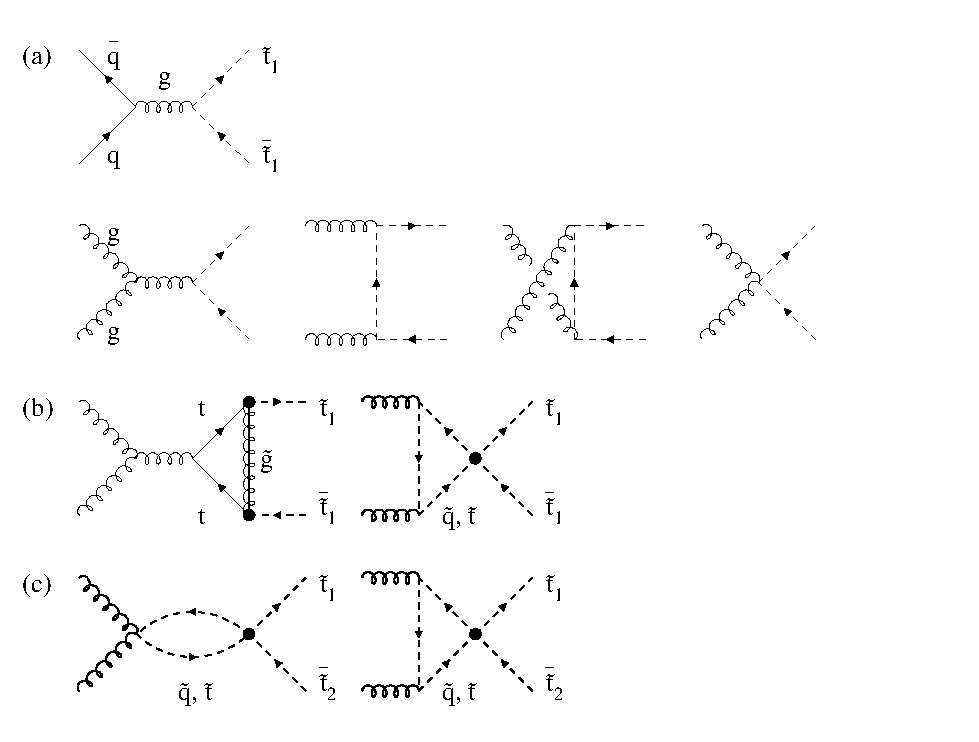
\includegraphics[trim=0.8cm 5.7cm 0cm 0cm, clip=true, width=0.995\textwidth]{BeyondSM/Figures/feyn_fin.eps}
}
\end{center}
\caption[Born diagrams for quark-antiquark annihilation and gluon fusion, leading to pairs of stop particles.]{Born diagrams for quark-antiquark annihilation and gluon fusion, leading to pairs of stop particles~\cite{Beenakker:1997ut}.}
\label{fig:StopProductionDiagrams}
\end{figure}

\begin{equation}
\begin{split}
\sigma_{q\bar{q} \rightarrow \tilde{q}_k\bar{\tilde{q}}_k} &= \frac{\alpha_s^2 \pi}{s} \frac{2}{27} \beta_k^3 \\
\sigma_{gg \rightarrow \tilde{q}_k \bar{\tilde{q}}_k} &= \frac{\alpha_s^2 \pi}{s} \left\{ \beta_k \left( \frac{5}{48} + \frac{31 m_{\tilde{q}_k}^2}{24s}\right) + \left(\frac{2m_{\tilde{q}_k}^2}{3s} + \frac{m_{\tilde{q}_k}^4}{6s^2}\right)\log{\left(\frac{1-\beta_k}{1+\beta_k}\right)} \right\} ,
\end{split}
\label{eq:StopSbottomCrossSection}
\end{equation}

\noindent where $k=1, 2$, $\squark = \stop, \sbottom$ and $\beta_k = \sqrt{1 - 4m_{\tilde{q}_k/s}}$.
Different simplified models are considered involving production of third generation squarks in the analysis presented in this Thesis:

\begin{itemize}
\item{Stop pair production with $\stoptocharm$:} The gluino together with the first and second squark generations are decoupled from the theory.
\item{Stop pair production with $\stopfourbody$:} Same prescription as stop pair production with $\stoptocharm$.
\item{Sbottom pair production with $\sbottomtob$:} Same prescription as stop pair production with $\stoptocharm$.
\end{itemize}

Figure \ref{fig:Diagrams3rdGen} shows the Feynman diagrams for these three processes.

\begin{figure}[!ht]
\begin{center}
\mbox{
\includegraphics[width=0.3\textwidth]{BeyondSM/Figures/stst-ccN1N1-bWC1loop.eps}
\includegraphics[width=0.3\textwidth]{BeyondSM/Figures/stst-blvblvN1N1-4body.eps}
\includegraphics[width=0.3\textwidth]{BeyondSM/Figures/sbsb-bbN1N1.eps}
}
\end{center}
\caption[Feynman diagrams for different stop and sbottom pair production processes.]{Feynman diagrams for the direct stop and sbottom production processes studied. Left: stop pair production, with the stops decaying each to a charm quark and a neutralino. Center: Stop pair production with the stops decaying each to a bottom quark, two fermions and a neutralino. Right: sbottom pair production, each decaying to a bottom quark and a neutralino.}
\label{fig:Diagrams3rdGen}
\end{figure}


\subsubsection{Squark and gluino production}

The hadroproduction of squarks and gluinos at leading order, whose Feynman diagrams and cross section computations are shown in Figure~\ref{fig:SquarkGluinoProductionDiagrams} and in Ref.~\cite{Beenakker:1996ch}, respectively, proceeds through the following partonic interactions:

\begin{figure}[!ht]
\begin{center}
\mbox{
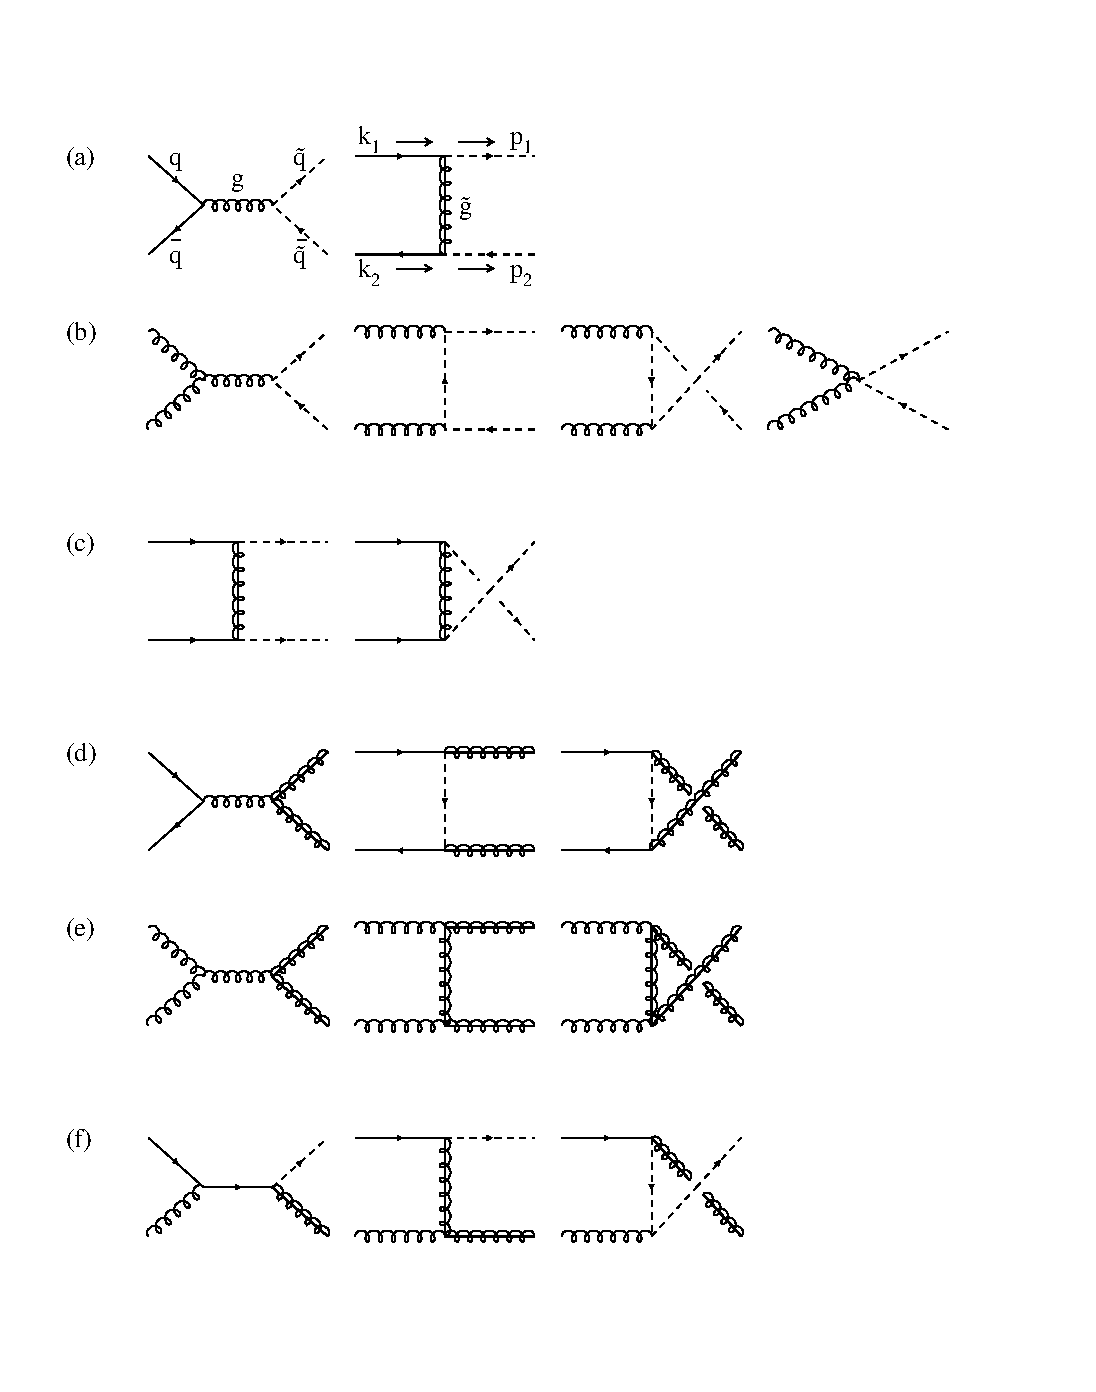
\includegraphics[width=0.995\textwidth]{BeyondSM/Figures/bornfeyn.eps}
}
\end{center}
\caption[Feynman diagrams for the production of squarks and gluinos in lowest order.]{Feynman diagrams for the production of squarks and gluinos in lowest order. The diagrams without and with crossed final-state lines represent $t-$ and $u-$ channel diagrams, respectively. The diagrams in (c) and the last diagram in (d) are a result of the Majorana nature of gluinos. Note that some of the above diagrams contribute only for specific flavors and chiralities of the squarks~\cite{Beenakker:1996ch}.}
\label{fig:SquarkGluinoProductionDiagrams}
\end{figure}

\begin{equation}
\begin{matrix}
\tilde{q} \bar{\tilde{q}} \text{ production: } & q_i + \bar{q}_j &\rightarrow & \tilde{q}_k + \bar{\tilde{q}}_l & \\
& g   + g         &\rightarrow & \tilde{q}_k + \bar{\tilde{q}}_l & \\
\tilde{q} \tilde{q} \text{ production: }       & q_i + q_j       &\rightarrow & \tilde{q}_k + \tilde{q}_l & \text{ and } c.c.\\
\tilde{g} \tilde{g} \text{ production: }       & q_i + \bar{q}_i &\rightarrow & \tilde{g}   + \tilde{g} & \\
& g   + g         &\rightarrow & \tilde{g}   + \tilde{g} & \\
\tilde{q} \tilde{q} \text{ production: }       & q_i + g         &\rightarrow & \tilde{q}_i + \tilde{g} & \text{ and } c.c.
\end{matrix}
\label{eq:DirectSquarkGluinoProduction}
\end{equation}

In this picture, the chiralities of the squarks are not considered explicitly, $\squark = (\squark_L, \squark_R)$, and the indices $i$-$l$ indicate the flavors of the quarks and squarks involved.
In the analysis, only first and second squark generations are considered, degenerated in mass. 

The following simplified models are considered for analysis, while the Feynman diagrams for these processes are shown in Figure~\ref{fig:DiagramsInclusiveProduction}:

\begin{itemize}
\item{Squark pair production with $\squarktoq$: }The third generation squarks and the gluino masses are set to $\unit[5]{TeV}$ and therefore are decoupled from the theory.
\item{Gluino pair production with $\gluinotog$: }Assumed 100\% branching ratio for this decay, with the rest of SUSY particles decoupled, but the neutralino.
\item{Gluino pair production with $\gluinotobb$: }Same prescription as gluino pair production with $\gluinotog$.
\end{itemize}

\begin{figure}[!ht]
\begin{center}
\mbox{
\includegraphics[width=0.3\textwidth]{BeyondSM/Figures/sqsq-qqN1N1.eps}
\includegraphics[width=0.3\textwidth]{BeyondSM/Figures/gogo-ggN1N1.eps}
\includegraphics[width=0.3\textwidth]{BeyondSM/Figures/gogo-bbbbN1N1.eps}
}
\end{center}
\caption[Feynman diagrams for different inclusive squark/gluino production processes.]{Feynman diagrams for the inclusive squark/gluino production processes studied. Left: inclusive squark pair production, with the squarks decaying each to a quark and a neutralino. Center: gluino pair production with the gluino decaying each to a gluon and a neutralino. Right: gluino pair production, each decaying to a bottom and antibottom quarks and a neutralino.}
\label{fig:DiagramsInclusiveProduction}
\end{figure}


\subsubsection{Processes involving direct production of charginos or neutralinos}

SUSY electroweak particles are usually produced in the cascade decays.
However, they can also be produced directly in electroweak-driven processes, with much lower cross sections in comparison to SUSY strong production~\cite{Kramer:2012bx, Berggren:2013bua}.
In the analysis presented, two simplified model processes involving electroweakinos (whose Feynman diagrams are shown in Figure~\ref{fig:DiagramsElectroweakProduction}) are studied:

\begin{itemize}
\item{$\squarkneutralino$ production: } First and second squark generations are degenerated in mass, while the third generation squarks and the gluino are decoupled from the theory.
\item{$\charginoneutralino$ and $\charginochargino$ production: } All squarks, sleptons and gluino masses are set to more than $\unit[5]{TeV}$.
\end{itemize}

\begin{figure}[!ht]
\begin{center}
\mbox{
\includegraphics[width=0.3\textwidth]{BeyondSM/Figures/sqN1-qN1N1.eps}
\includegraphics[width=0.3\textwidth]{BeyondSM/Figures/C1C1-llvvN1N1-WW.eps}
\includegraphics[width=0.3\textwidth]{BeyondSM/Figures/C1N2-lllvN1N1-slsl.eps}
}
\end{center}
\caption[Feynman diagrams for processes involving the direct production of a chargino or a neutralino.]{Feynman diagrams for the electroweak SUSY production processes studied. Left: squark-neutralino production, with the squark decaying to a quark and a neutralino. Center: chargino pair production. Right: Chargino-neutralino production.}
\label{fig:DiagramsElectroweakProduction}
\end{figure}


\section{ADD Large Extra Dimensions}
\label{sec:ADD}

The Arkani-Hamed-Dimopoulos-Dvali \cite{ArkaniHamed:1998rs} (ADD) model of large extra dimensions is a framework which aims to solve the hierarchy problem without relying in supersymmetry.
In particular, this model provides an explanation to the 16 orders of magnitude difference between the electroweak and the Planck scales.
With this objective, $n$ extra spatial compactified dimensions with radius $R$ are added to the $3+1$ space-time dimensions.
Under this assumption, two test masses $m_1$ and $m_2$ placed at a distance $r\muchless R$ would feel a gravitational potential,

\begin{equation}
V(r) \sim \frac{m_1 m_2}{M^{n+2}_D} \frac{1}{r^{n+1}},\;\; (r\muchless R),
\label{eq:ADDPotentialrSmall}
\end{equation}

\noindent where $M_D$ is the Planck scale assuming $n$ extra dimensions.
However, if $r\gg R$,

\begin{equation}
V(r) \sim \frac{m_1 m_2}{M^{n+2}_D} \frac{1}{R^n r},\;\; (r\gg R),
\label{eq:ADDPotentialrBig}
\end{equation}

\noindent which can be related to the Newtonian gravitational potential:

\begin{equation}
V(r) \sim \frac{m_1 m_2}{M^2_P} \frac{1}{r},
\label{eq:ADDPotentialNewton}
\end{equation}

\noindent if the ``effective'' 4-dimensional Planck scale is equivalent to

\begin{equation}
M_P^2 \sim M_D^{2+n} R^n.
\label{eq:ADDPlanckMassEquivalence}
\end{equation}

In the ADD model, the electroweak scale $m_{EW}$ is the only fundamental short scale in nature.
Therefore, if $M_D \sim m_{EW}$, Equation~\ref{eq:ADDPlanckMassEquivalence} leads to:

\begin {equation}
R \sim 10^{\frac{30}{n}-17} \unit[]{cm} \times \left(\frac{\unit[1]{TeV}}{m_{EW}}\right).
\label{eq:ADDRRelation}
\end{equation}

This result points to the fact that $M_D$, the truth strength of the gravitational interaction can be as low as the electroweak scale providing values of $R$ as large as a millimeter.
For $n=1$, $R\sim \unit[10^{13}]{cm}$, which should produce deviations from Newtonian gravity over solar system distances, and therefore is empirically excluded.
For $n=2$, $R\sim \unit[100]{\mu m} - \unit[1]{mm}$, thus leading to deviations in the gravitational predictions that could be proved in the upcoming years\footnote{At present, gravity has been proven at the level of several hundreds of micrometers.}.
Higher $n$ values would lead to lower compactification radii $R$.

In the ADD model, the SM particles can only propagate in a 4-dimensional submanifold, while gravitons, understood as excitations of the $n$-dimensional metric, are the only particles allowed to $4+n$ dimensional bulk.

In terms of 4-dimensional indices, the metric tensor contains spin-2, spin-1 and spin-0 particles, which can be expressed as a tower of Kaluza-Klein modes \cite{KaluzaArticle,KleinArticle}.
The mass of each Kaluza-Klein mode corresponds to the modulus of its momentum in the direction transverse to the 4-dimensional brane.
In fact, the picture of a massless graviton propagating in a $n$-dimensional space or a massive Kaluza-Klein tower of massive gravitons propagating in a 4-dimensional space is completely equivalent.
At low energy and small curvature, the equations of motion of the effective theory reduce to Einstein equation in $n=4+\delta$ dimensions:

\begin{equation}
\mathcal{G}_{AB} \equiv \mathcal{R}_{AB} - \frac{1}{2} g_{AB}\mathcal{R} = - \frac{T_{AB}}{\bar{M}^{2+\delta}_D} \quad\quad A,B = 1,\ldots,n,
\label{eq:ADDEinsteinEquation}
\end{equation}

\noindent where $\bar{M}_D$ is the reduced Planck scale of the $n$-dimensional theory, $M_D = (2\pi)^{\delta/(2+\delta)} \bar{M}_D$.
If the metric $g_{AB}$ is expanded around its Minkowski value $\eta_{AB}$,

\begin{equation}
g_{AB} = \eta_{AB} + 2 \bar{M}_D^{-1-\delta/2}h_{AB},
\label{eq:ADDMinkowskiExpansion}
\end{equation}

\noindent Equation~\ref{eq:ADDEinsteinEquation} can then be rewritten as:

\begin{equation}
\begin{split}
\bar{M}_D^{1+\delta/2} \mathcal{G} &= \Box h_{AB} - \partial_A \partial^C h_{CB} - \partial_B \partial^C h_{CA} + \partial_A \partial_B h^C_C \\
&- \eta_{AB} \Box h_C^C + \eta_{AB}\partial^C \partial^D h_{CD} = - \bar{M}_D^{-1-\delta/2} T_{AB},
\end{split}
\label{eq:ADDEinsteinEquationPowersH}
\end{equation}

\noindent keeping only the first power of $h$.
The previous expression can be derived from the following $n$-dimensional graviton lagrangian:

\begin{equation}
\begin{split}
\lagrangian_{\text{grav}} &= -\frac{1}{2}h^{AB} \Box h_{AB} + \frac{1}{2}h^A_A \Box h^B_B \\
&- h^{AB} \partial_A \partial_B h_C^C + h^{AB} \partial_A \partial_C h_B^C - \frac{1}{\bar{M}_D^{-1-\delta/2}} h^{AB} T_{AB}.
\end{split}
\label{eq:ADDGravitonLagrangian}
\end{equation}

This lagrangian becomes the sum over the Kaluza-Klein modes of:

\begin{equation}
\begin{split}
\lagrangian_{\text{grav}} &= \sum_{\text{all }\vec{n}} -\frac{1}{2} G^{(-\vec{n})\mu\nu} (\Box + m^2)G^{(-\vec{n})}_{\mu\nu} + \frac{1}{2} G^{(-\vec{n})\mu}_{\mu} (\Box + m^2) G^{(-\vec{n})\nu}_{\nu} \\
&- G^{(\vec{n})\mu\nu} \partial_\mu \partial_\nu G^{(\vec{n})\lambda}_{\lambda} + G^{(\vec{n})\mu\nu} \partial_\mu \partial_\lambda G^{(\vec{n})\lambda}_{\nu} - \frac{1}{M_P}G^{(\vec{n})\mu\nu}T_{\mu\nu}, \\
&+ \cdots \\
\end{split}
\label{eq:ADDGravitonLagrangian4D}
\end{equation}

\noindent under the unitary gauge and the parametrization from Reference~\cite{Giudice:1998ck}.
In this equation, the ellipses refer to spin-2, spin-1 and spin-0 particles that are not coupled (or their coupling is very suppressed) to the SM energy-momentum tensor $T_{\mu\nu}$, and therefore play no role in a collider experiment.
The latest term is the graviton interaction lagrangian.
If $T_{\mu\nu}$ is expanded, the Feynman rules for the interactions between gravitons and SM fields can be retrieved.

For not very high $\delta$ (i.e. $\delta \lesssim 6$) the mass difference between the graviton modes is small and the contributions of the different modes can be integrated over the mass.
Under this approximation, the differential cross section for inclusive graviton production is expressed as:

\begin{equation}
\frac{d^2\,\sigma}{dt\; dm} = \frac{2\pi^{\delta/2}}{\Gamma(\delta/2)} \frac{M_P^2}{M_D^{2+\delta}} m^{\delta-1} \frac{d\, \sigma_m}{dt},
\label{eq:ADDCrossSectionmass}
\end{equation}

\noindent where $d\sigma_m/dt$ is the differential cross section for producing a single Kaluza-Klein graviton of mass $m$, found to be:

\begin{equation}
\begin{split}
\frac{d\sigma_m}{dt}(q\bar{q} \rightarrow gG) &= \frac{\alpha_s}{36}\frac{1}{M_P^2 s}F_1(t/s, m^2/s) \\
\frac{d\sigma_m}{dt}(qg \rightarrow qG) &= \frac{\alpha_s}{96}\frac{1}{M_P^2 s}F_2(t/s, m^2/s)\\
\frac{d\sigma_m}{dt}(gg \rightarrow gG) &= \frac{3\alpha_s}{16}\frac{1}{M_P^2 s}F_3(t/s, m^2/s),
\end{split}
\label{eq:ADDCrossSectionIndividualProcess}
\end{equation}

\noindent with the expressions $F_1$, $F_2$ and $F_3$ reported in Reference~\cite{Giudice:1998ck}.
Figure \ref{fig:DiagramsADDProduction} shows the Feynman diagrams for the graviton production at colliders at LO.

The ADD model is an effective theory and therefore, it is only valid up to a given scale, which is assumed to be of the order of $m_{EW}$.
For this reason, the effects of the hypothetical underlying theory are expected to emerge at energy scales close to $M_D$.

\begin{figure}[!ht]
\begin{center}
\mbox{
\includegraphics[width=0.3\textwidth]{BeyondSM/Figures/ADD_gggG.eps}
\includegraphics[width=0.3\textwidth]{BeyondSM/Figures/ADD_qqgG.eps}
\includegraphics[width=0.3\textwidth]{BeyondSM/Figures/ADD_qgqG.eps}
}
\mbox{
\includegraphics[width=0.3\textwidth]{BeyondSM/Figures/ADD_ggggG.eps}
\includegraphics[width=0.3\textwidth]{BeyondSM/Figures/ADD_qgqqG.eps}
}
\end{center}
\caption{Feynman diagrams for the Kaluza-Klein graviton production.}
\label{fig:DiagramsADDProduction}
\end{figure}


\section{Dark Matter and WIMPs}
\label{sec:WIMPs}

The existence of non-luminous matter called ``dark matter'' (DM) in the Universe (see Ref.~\cite{Bertone:2004pz} for a complete review), is inferred from the observation of its gravitational interactions and is well-motivated by experimental observations.
The most convincing evidence for dark matter on galactic scales comes from the observations of the velocity of rotation of stars and gas in spiral galaxies.
If these galaxies were composed only of luminous matter, the circular velocity would be $v(r)\propto 1/\sqrt{r}$ beyond the optical disc.
The fact that $v(r)$ is observed to be approximately constant implies the existence of an halo of DM three to ten times larger than that corresponding to the visible matter, that interacts gravitationally, as shown in Figure \ref{fig:DMProofVelocityStars}.

\begin{figure}[!ht]
\begin{center}
\mbox{
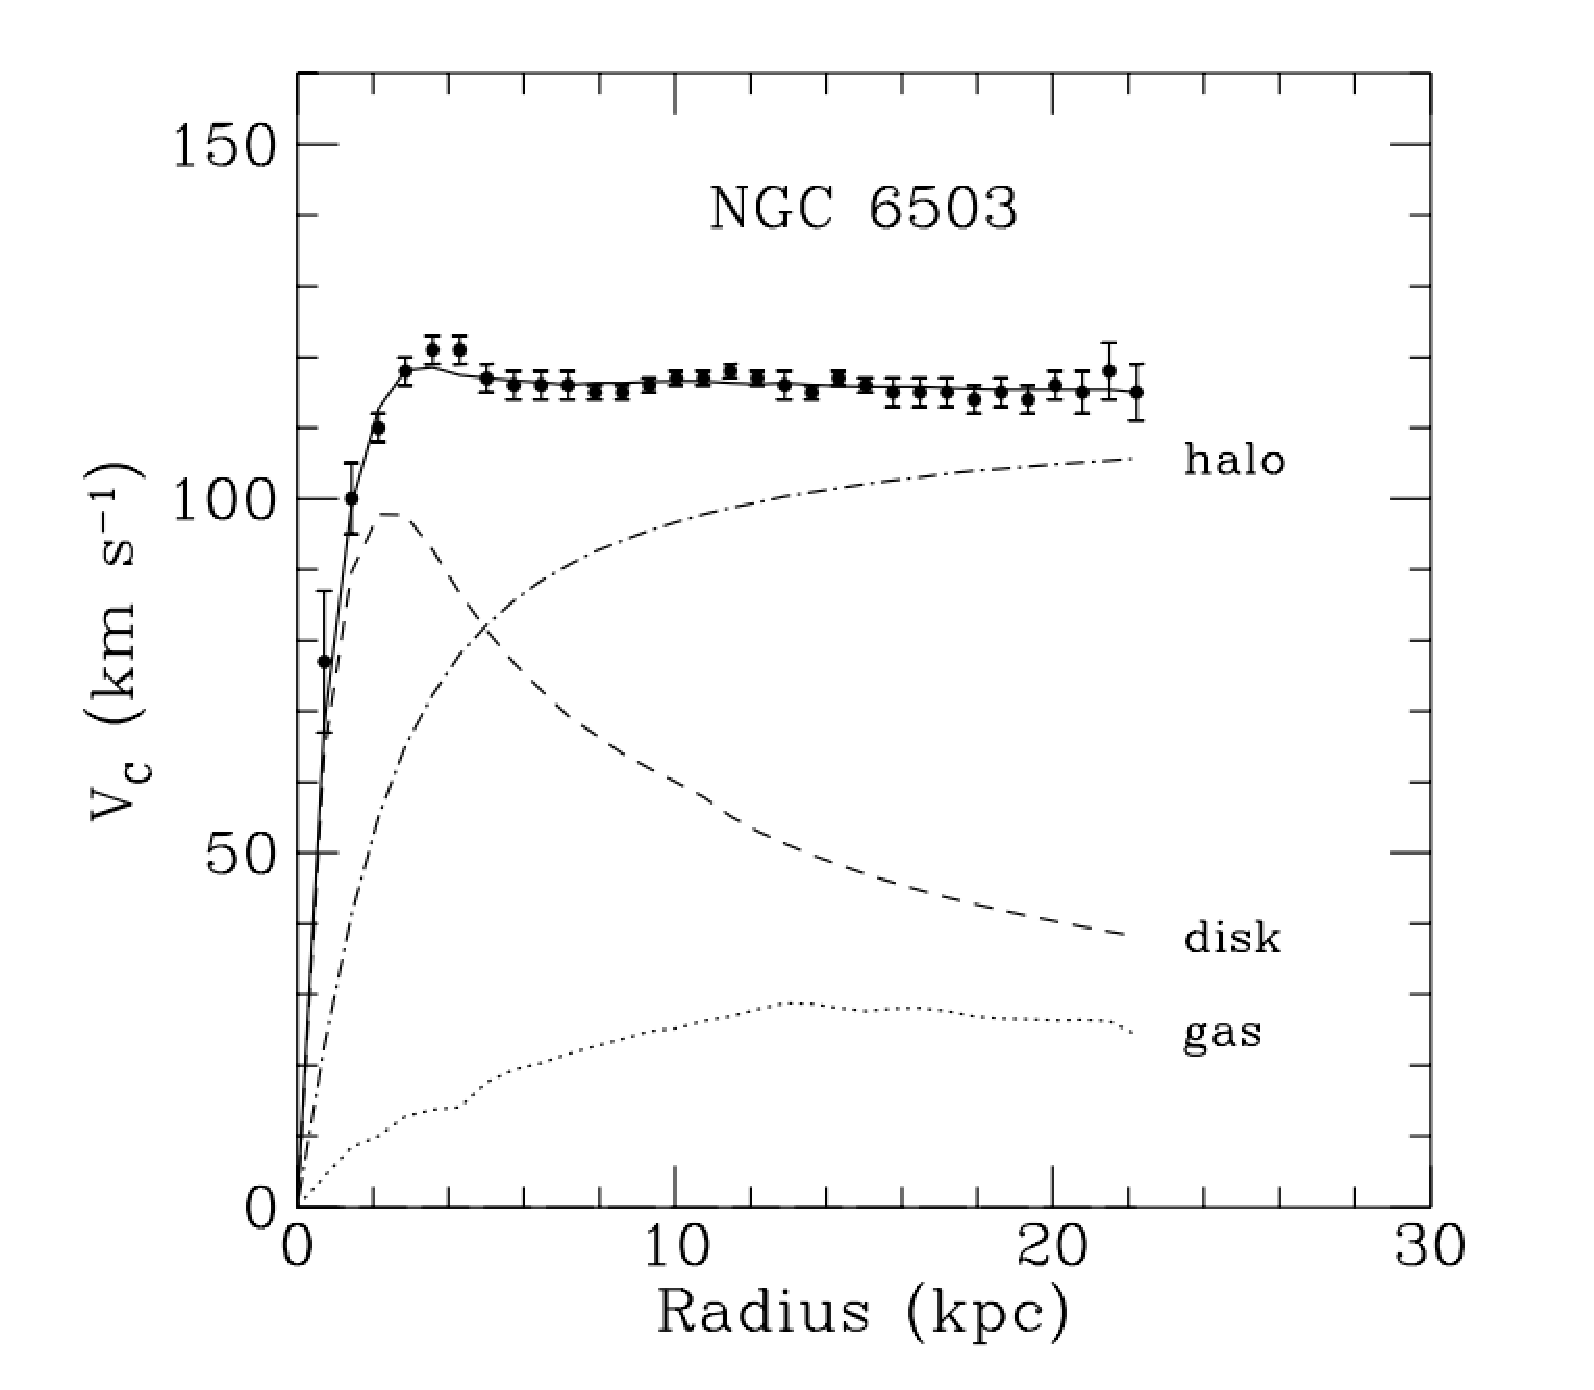
\includegraphics[width=0.495\textwidth]{BeyondSM/Figures/GalaxyVelocityRotation.eps}
}
\end{center}
\caption[Rotational velocity of stars as a function of the radius in the spiral galaxy NGC6503.]{Rotational velocity of stars as a function of the radius in the spiral galaxy NGC6503. The dotted, dashed and dash-dotted lines are the contributions of gas, disk and dark matter, respectively \protect\cite{Begeman:1991iy}.}
\label{fig:DMProofVelocityStars}
\end{figure}

Other evidences for the existence of DM come from a great variety of data, like the strong gravitational lensing.
Weak modulation of strong lensing around individual massive elliptical galaxies \cite{Metcalf:2003sz}, weak gravitational lensing of distant galaxies by foreground structure \cite{Hoekstra:2002nf}, or studies on the velocity dispersions of dwarf spheroidal galaxies \cite{Metcalf:2003sz} also suggest the presence of Dark Matter.

The measurement of the ``cosmic microwave background'' (CMB) also points to the existence of DM. 
The CMB is the thermal radiation background that is measured in the Universe, corresponding to roughly $\unit[2.7]{K}$ of temperature.
It is known to be isotropic at the $10^{-5}$ level.
The CMB is not associated to any specific object, but to the propagation of photons once they were decoupled from matter about $\unit[3.5 \times 10^5]{years}$ after the Big Bang.
A detailed study of the angular correlation in the CMB fluctuations gives information about the geometry of the Universe, about its evolution and its energy-matter content.
Many measurements of the CMB radiation have been performed along the years, the most stringent ones done by the WMAP and the PLANCK experiments~\cite{Larson:2010gs,Ade:2013zuv}.
From these measurements it can be inferred the presence of much larger quantities of dark matter in the early Universe.
A striking coincidence in cosmology is that if DM would annihilate to SM particles with an interaction strength close to that of the weak force, that would result exactly in the decrease of DM density observed between the early and the present Universes.
This coincidence leads to the idea that DM could be composed of Weakly Interacting Massive Particles (WIMPs)~\cite{Zacek:2007mi}.

None of the known SM particles are adequate DM candidates, and for this reason, the existence of a new particles is often hypothesized.
WIMPs, with masses roughly between $\unit[10]{GeV}$ and a few TeV, are one of such class of particle candidates.
They are expected to couple to SM particles through a generic weak interaction, which could be the known weak interaction of the SM or a new type of interaction.
A variety of detection techniques have been developed along the years to search WIMPs, which can be classified depending on the kind of process that they are aimed to observe.
Direct detection experiments aim to observe WIMP-nucleon elastic scattering by measuring the nuclear recoil.
In the last decade, several published results from the direct detection experiments DAMA/LIBRA\cite{Bernabei:2010mq}, CDMS II\cite{Agnese:2013rvf}, CRESST-II\cite{Angloher:2011uu} and CoGent\cite{Aalseth:2010vx} pointed to the existence of light ($\sim\unit[10]{GeV}$) WIMP particles, although these results have been challenged by several other experiments, such as XENON100\cite{Aprile:2012nq}.
Instead, indirect detection experiments search for the SM products from the WIMP-WIMP annihilation.
Finally, collider searches allow the direct production of WIMPs from the annihilation of SM particles.
The sensitivity of collider searches is comparable to the direct and indirect detection searches, especially for low mass WIMPs, since the recoil that the SM particle receives is smaller as the mass of the WIMP decreases.


\subsection{Effective Theory models}

The interaction of WIMPs with SM particles is described as a contact interaction using an effective field theory (EFT) approach, as mediated by a single new heavy particle with mass too large to be produced directly at the LHC.
The use of a contact interaction to produce WIMP pairs via heavy mediators is considered conservative because it rarely overestimates cross sections when applied to a specific BSM scenario.
In this Thesis, WIMPs are assumed to be Dirac-like fermions, and to be odd under the $Z_2$ symmetry, so that each coupling involves an even number of WIMPs.
Different effective operators (described in Table \ref{tab:WIMPsEffectiveOperators}) are considered to describe different bilinear quark couplings to WIMPs.

\begin{table}[tb]
\begin{center}
\begin{tabular}{|cc|cc|}
\hline
\textbf{Name} & \textbf{Operator} & \textbf{Name} & \textbf{Operator} \\
\hline
D1  & $\frac{m_q}{(M^{\ast})^3} \bar{\chi}\chi \bar{q}q$                                         & D2  & $\frac{m_q}{(M^{\ast})^3} \bar{\chi} \gamma^5 \chi \bar{q}q$ \\
D3  & $\frac{m_q}{(M^{\ast})^3} \bar{\chi}\chi \bar{q}\gamma^5 q$                                & D4  & $\frac{m_q}{(M^{\ast})^3} \bar{\chi} \gamma^5 \chi \bar{q} \gamma^5 q$ \\
D5  & $\frac{1}{(M^{\ast})^2} \bar{\chi}\gamma^{\mu} \chi \bar{q} \gamma_{\mu} q$                & D6  & $\frac{1}{(M^{\ast})^2} \bar{\chi}\gamma^{\mu}\gamma^5 \chi \bar{q} \gamma_{\mu} q$ \\
D7  & $\frac{1}{(M^{\ast})^2} \bar{\chi}\gamma^{\mu} \chi \bar{q} \gamma_{\mu} \gamma^5 q$       & D8  & $\frac{1}{(M^{\ast})^2} \bar{\chi}\gamma^{\mu}\gamma^5 \chi \bar{q} \gamma_{\mu} \gamma^5 q$ \\
D9  & $\frac{1}{(M^{\ast})^2} \bar{\chi}\sigma^{\mu\nu} \chi \bar{q} \sigma_{\mu\nu} \gamma^5 q$ & D10 & $\frac{1}{(M^{\ast})^2} \epsilon^{\mu\nu\alpha\beta}\bar{\chi}\sigma_{\mu\nu} \chi \bar{q} \sigma_{\alpha\beta} \gamma^5 q$ \\
D11 & $\frac{1}{(4 M^{\ast})^3} \bar{\chi}\chi \alpha_s (G^a_{\mu\nu})^2$                        & D12 & $\frac{1}{(4 M^{\ast})^3} \bar{\chi} \gamma^5 \chi \alpha_s (G^a_{\mu\nu})^2$ \\
D13 & $\frac{1}{(4 M^{\ast})^3} \bar{\chi}\chi \alpha_s G^a_{\mu\nu} \tilde{G}^{a,\mu\nu}$       & D14 & $\frac{1}{(4 M^{\ast})^3} \bar{\chi} \gamma^5 \chi \alpha_s G^a_{\mu\nu} \tilde{G}^{a,\mu\nu}$ \\
\hline
\end{tabular}
\end{center}
\caption[Effective operators involving couplings between Dirac-like fermion WIMPs and Standard Model quarks or gluons.]{Effective operators involving couplings between Dirac-like fermion WIMPs and Standard Model quarks or gluons~\protect\cite{Goodman:2010ku}.}
\label{tab:WIMPsEffectiveOperators}
\end{table}

In the operator definitions listed in this table, $M^{\ast}$ is the suppression scale of the interaction, after the heavy mediator particle has been integrated.
In the following, only the D5 (vector), D8 (axial-vector) and D9 (tensor) operators from Table~\ref{tab:WIMPsEffectiveOperators} will be considered.

The collider results can also be compared to direct detection experiments, since the WIMP-nucleon cross section is found to be~\cite{Goodman:2010ku}:

\begin{equation}
\begin{split}
\sigma^{D5}_{\chi N} &= 1.38 \times \unit[10^{-37}]{cm^2} \times \left(\frac{\mu_{\chi}}{\unit[1]{GeV}}\right)^2\left(\frac{\unit[300]{GeV}}{M^{\ast}}\right)^4 \\
\sigma^{D8}_{\chi N} &= 4.70 \times \unit[10^{-40}]{cm^2} \times \left(\frac{\mu_{\chi}}{\unit[1]{GeV}}\right)^2\left(\frac{\unit[300]{GeV}}{M^{\ast}}\right)^4 \\
\sigma^{D9}_{\chi N} &= 4.70 \times \unit[10^{-40}]{cm^2} \times \left(\frac{\mu_{\chi}}{\unit[1]{GeV}}\right)^2\left(\frac{\unit[300]{GeV}}{M^{\ast}}\right)^4, \\
\end{split}
\label{eq:WIMP-Nucleon}
\end{equation}

\noindent where $\mu_{\chi}$ is the reduced mass of the WIMP-nucleon system, $\mu_{\chi} = (m_{\chi} \times m_N) / (m_{\chi} + m_N)$.
In direct detection experiments, the typical transferred momentum is of the order of the keV and therefore, the propagator of a mediator with mass $M \gg \unit[1]{keV}$ cannot be resolved, thus making these effective theories suitable for this regime.
However, the LHC center of mass energy of the partons can be up to the TeV scale, and thus targeting a completely different phase space region.
This motivates the need to carefully study the validity of the EFT approach.


\subsection{Simplified models}
    \label{subsubsec:simplifiedModels}

The effective theory models previously introduced, are based on the assumption that the mediator mass is much higher than the scale of the interaction, and for this reason, it cannot be produced directly.
This assumption is not always correct at the LHC, where the momentum transfer can reach the TeV energies.

Instead, simplified models can be used to parametrize the interaction between the quarks and the WIMPs.
These interactions are mediated by a vector particle $Z'$ of a given mass $M_{\text{med}}$, with $\Gamma_{\text{med}}$, and couplings $g_{q}$ and $g_{\chi}$ to the SM particles and WIMPs, respectively.
